\documentclass{beamer}
\usepackage[utf8]{inputenc} 
\usepackage[T1]{fontenc}
\usepackage{hyperref}
\usepackage{colortbl}
\usepackage{tcolorbox}
\usepackage{fourier}
% \usepackage{biblatex}
% \addbibresource{references.bib}

% \usepackage[autostyle=true]{csquotes} % Required to generate language-dependent quotes in the bibliography

% other packages
\usepackage{latexsym,amsmath,xcolor,multicol,booktabs,calligra,mathpazo}
\usepackage{graphicx,listings,stackengine}
\usepackage{subcaption}
\usepackage{caption}
\usepackage{xcolor}
\usepackage{colortbl}
\usepackage{tabularx}
\usepackage{tikz}
\usepackage{pifont}
\usepackage{cancel}

% TABULAR DEFINITIONS

\renewcommand\tabularxcolumn[1]{m{#1}}  % vertical centering of text in tabularx 
\newcommand\Mark[2][8.4]{%
	\rlap{\tikz[baseline=(current bounding box.south)]{
			\shade[left color=red, right color=green!#2!red]
			(0,0) rectangle ++(#1*#2/100,0.3);}%
	}%
}

% OTHER DEFINITIONS

\definecolor{vtxtablegray}{RGB}{208, 213, 215}

\DeclareCaptionFormat{myformat}{\textbf{#1#2}#3}
 \captionsetup{format=myformat}

% MATHEMATICAL DEFINITIONS

\newcommand{\xmark}{\textcolor{red}{\ding{55}}} % Red cross

\newcommand{\R}{\mathbb{R}}
\renewcommand{\P}{\mathbb{P}}
\newcommand{\C}{\mathcal{C}}
\newcommand{\Ca}{\mathcal{C}_{\alpha}}
\renewcommand{\S}{\mathcal{S}}
\newcommand{\A}{\mathcal{A}}
\renewcommand{\a}{\alpha}
\newcommand\myeq{\mathrel{\stackrel{\makebox[0pt]{\mbox{\normalfont\tiny a.s.}}}{=}}}

% \author{Gerard Castro}

\title{Conformal prediction and beyond}
\subtitle{Uncertainty quantification for regression \& time-series problems}
\institute{% \includegraphics[width=0.025\linewidth]{Figures/ub.png}\vspace{5mm}\  
Universitat de Barcelona}
\author{Gerard Castro}
\date{\today}
\usepackage{slides}


% defs
\def\cmd#1{\texttt{\color{red}\footnotesize $\backslash$#1}}
\def\env#1{\texttt{\color{blue}\footnotesize #1}}
\definecolor{deepblue}{rgb}{0,0,0.5}
\definecolor{deepred}{rgb}{0.6,0,0}
\definecolor{deepgreen}{rgb}{0,0.5,0}
\definecolor{halfgray}{gray}{0.55}

\newcommand\checkitem{\item[\color{green}\checkmark]}
\newcommand\dangeritem{\item[\color{yellow}\danger]}
\newcommand\crossitem{\item[\color{red}\texttimes]}

\lstset{
    basicstyle=\ttfamily\small,
    keywordstyle=\bfseries\color{deepblue},
    emphstyle=\ttfamily\color{deepred},    % Custom highlighting style
    stringstyle=\color{deepgreen},
    numbers=left,
    numberstyle=\small\color{halfgray},
    rulesepcolor=\color{red!20!green!20!blue!20},
    frame=shadowbox,
}


\begin{document}

%%% TITLE & INITIAL FRAME %%%

\begin{frame}
    \titlepage
    \begin{figure}[htpb]
        \begin{center}
           
\includegraphics[width=0.4\linewidth]{Figures/fmiub.png}
        \end{center}
    \end{figure}
\end{frame}

%%%% OUTLINE %%%%
%%% - Introduction: 10% (2pp) 
%%% - Conformal prediction: %20 (4 pp)
%%% - Beyond exchangeability: 20% (4pp)
%%% - Results (8pp)
%% - Metrics: 5% (1p)
%% - Regression problem: 10% (2pp)
%% - Timeseries problem: 25% (5pp)

% - Conclusions: %10 (2pp)

%%% INTRODUCTION %%% (2pp)

\section{Introduction}

% MAIN IDEA %

\begin{frame}{Motivation}
    \begin{itemize}%[<+->]
        \item We extract $n$ samples from $(X, Y)\in \R^d\times\R$ random variables with unknown marginal \& joint distributions.
        \item Given a new sample $X_{n+1}$ \& miscoverage level $\a\in\left[ 0, 1\right]$: 
        \begin{itemize}%[<+->][<+->]  
            \item We want to \textbf{estimate} a predictive \textbf{interval} $\Ca$ such that the probability of $Y_{n+1}$ falling into $\Ca$ is at least $1-\a$, \textit{i.e.}
            \begin{equation*}
                \P \{ Y_{n+1} \in \Ca\left(X_{n+1}\right) \} \geq 1 - \a
            \end{equation*}
            \item The interval should be the \textbf{smallest} possible while \textbf{keeping coverage}. \textbf{Conditional} coverage ideally sought.
        \end{itemize} 
    
    %%% FIGURE %%%
    \item[]<2-> 
    \begin{figure}[ht]
        \centering
        \begin{subfigure}[b]{0.3\textwidth}
            \centering
            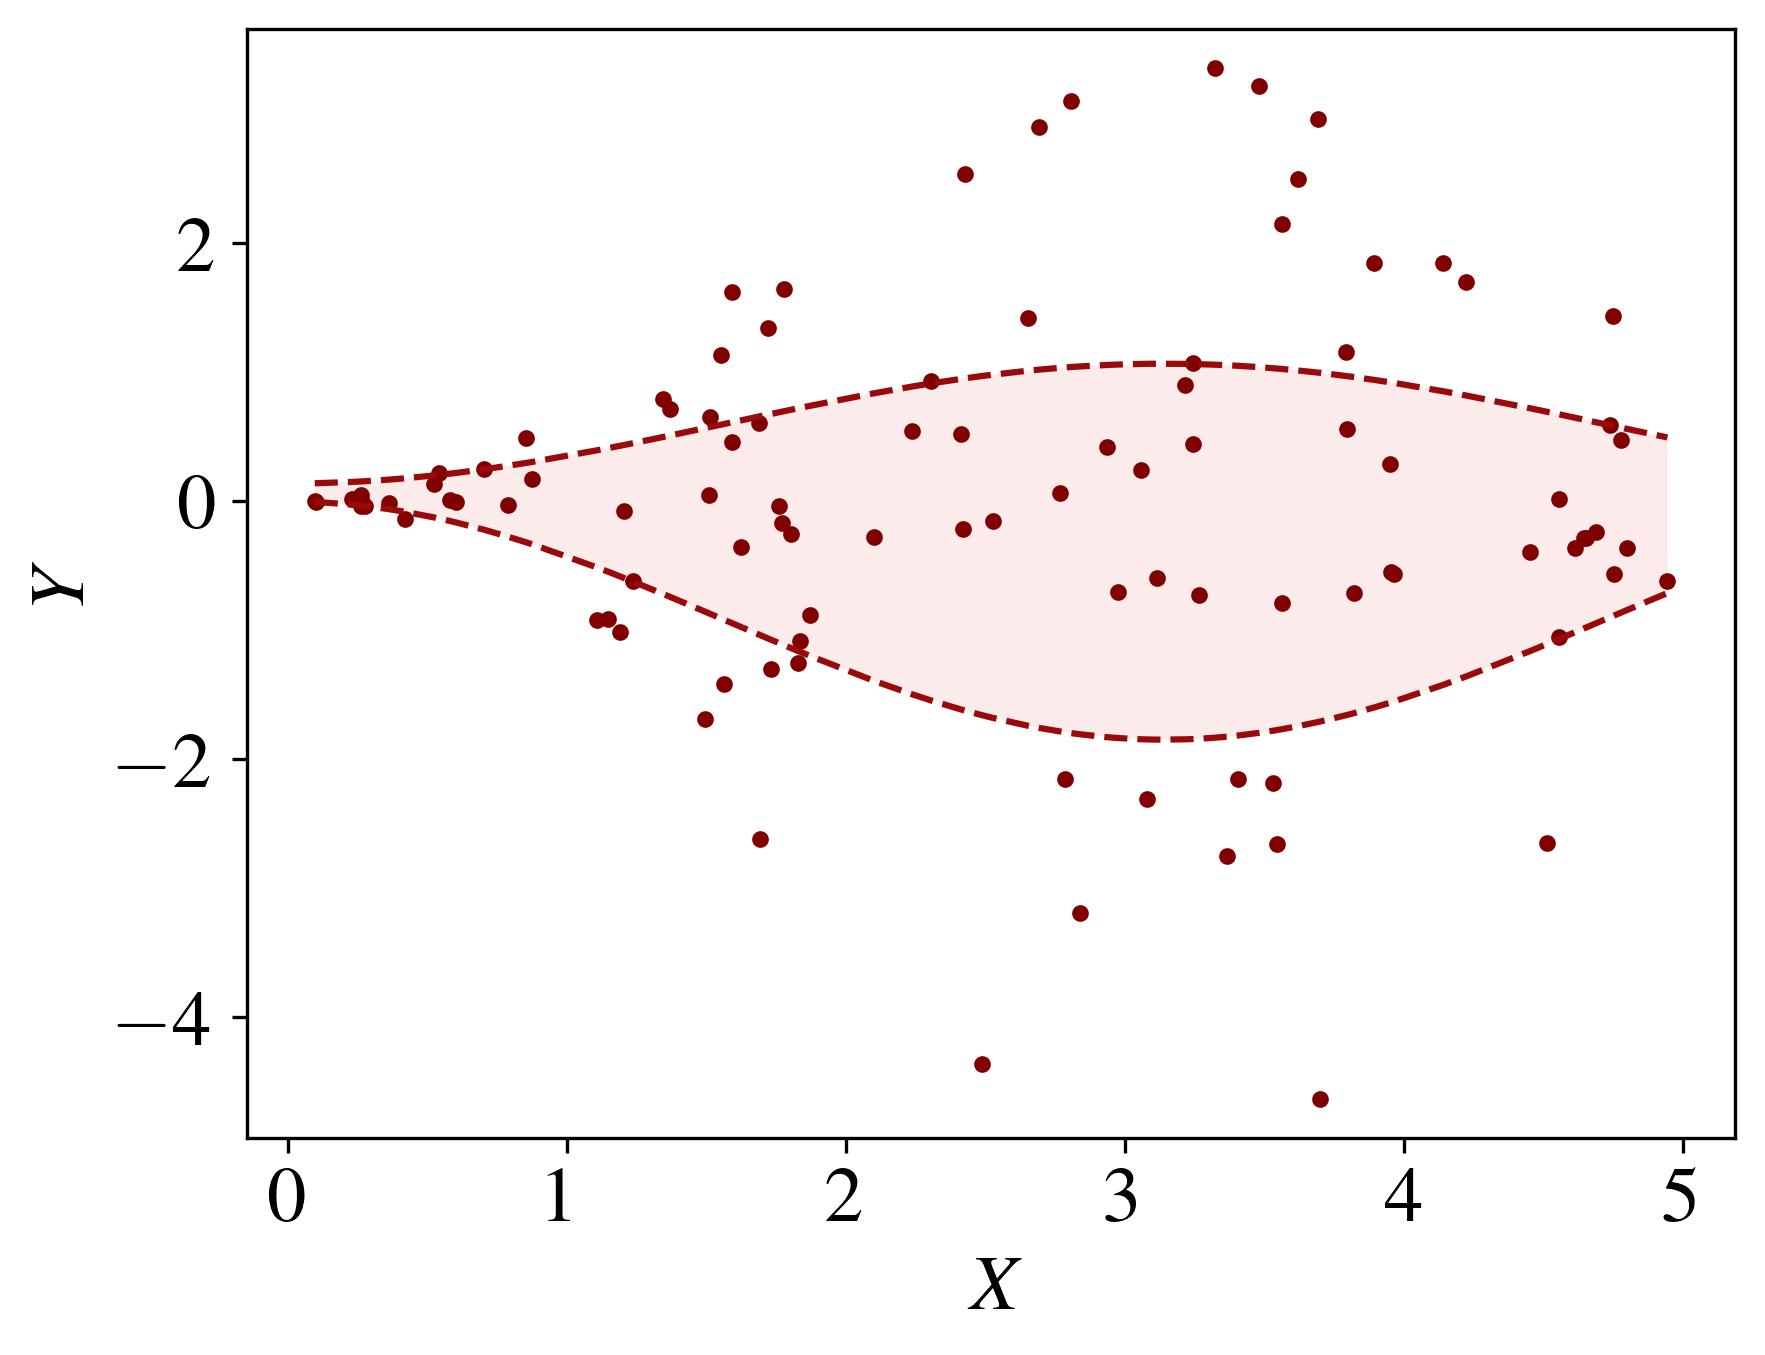
\includegraphics[width=\textwidth, height=0.55\textwidth]{Figures/coverage/no-coverage.png}
            \caption{No coverage}
            \label{fig:coverage:no-cover}
        \end{subfigure}
        \hfill
        \begin{subfigure}[b]{0.3\textwidth}
            \centering
            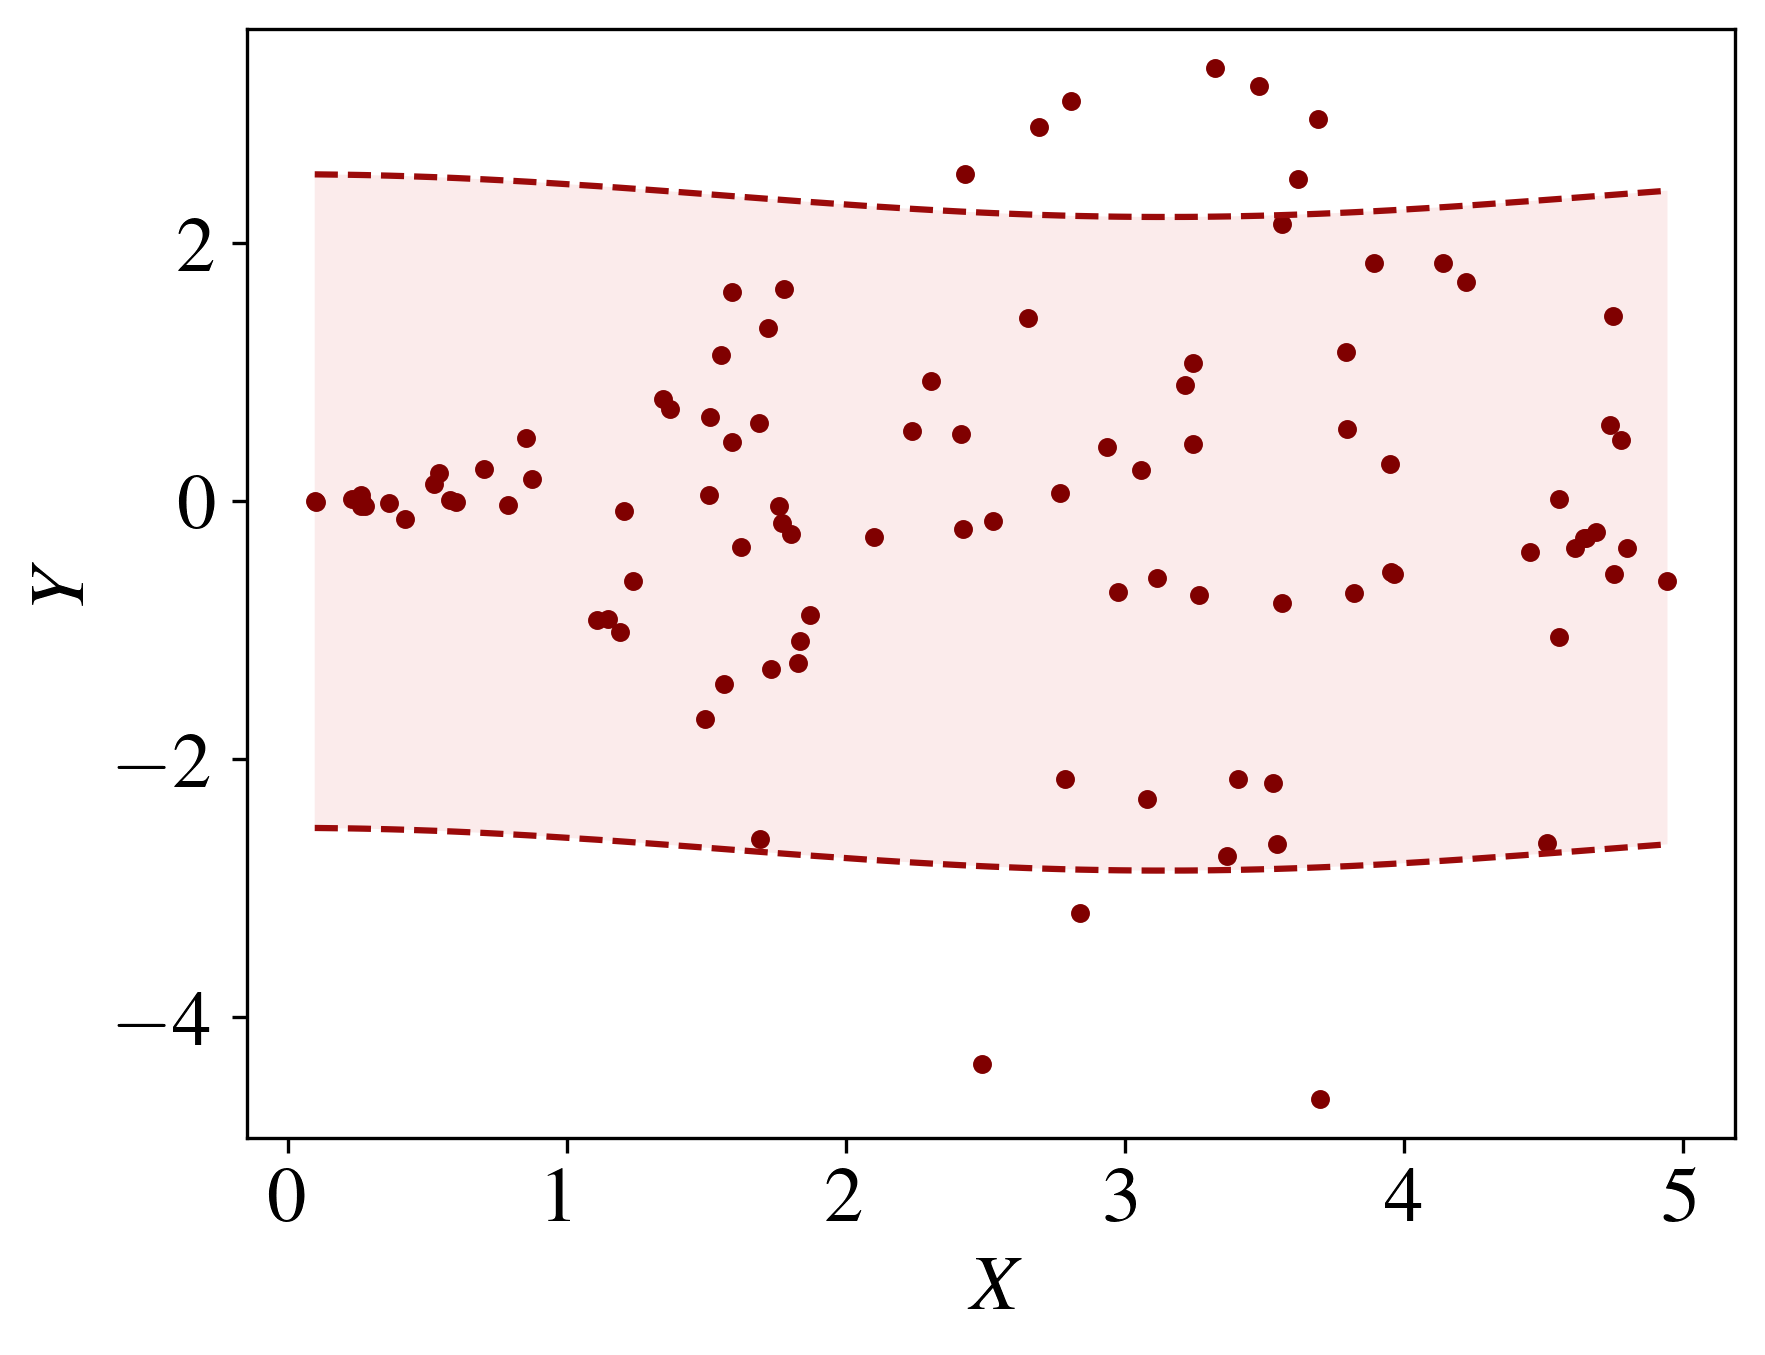
\includegraphics[width=\textwidth, height=0.55\textwidth]{Figures/coverage/marginal-coverage.png}
            \caption{Marginal coverage}
            \label{fig:coverage:marg-cover}
        \end{subfigure}
        \hfill
        \begin{subfigure}[b]{0.3\textwidth}
            \centering
            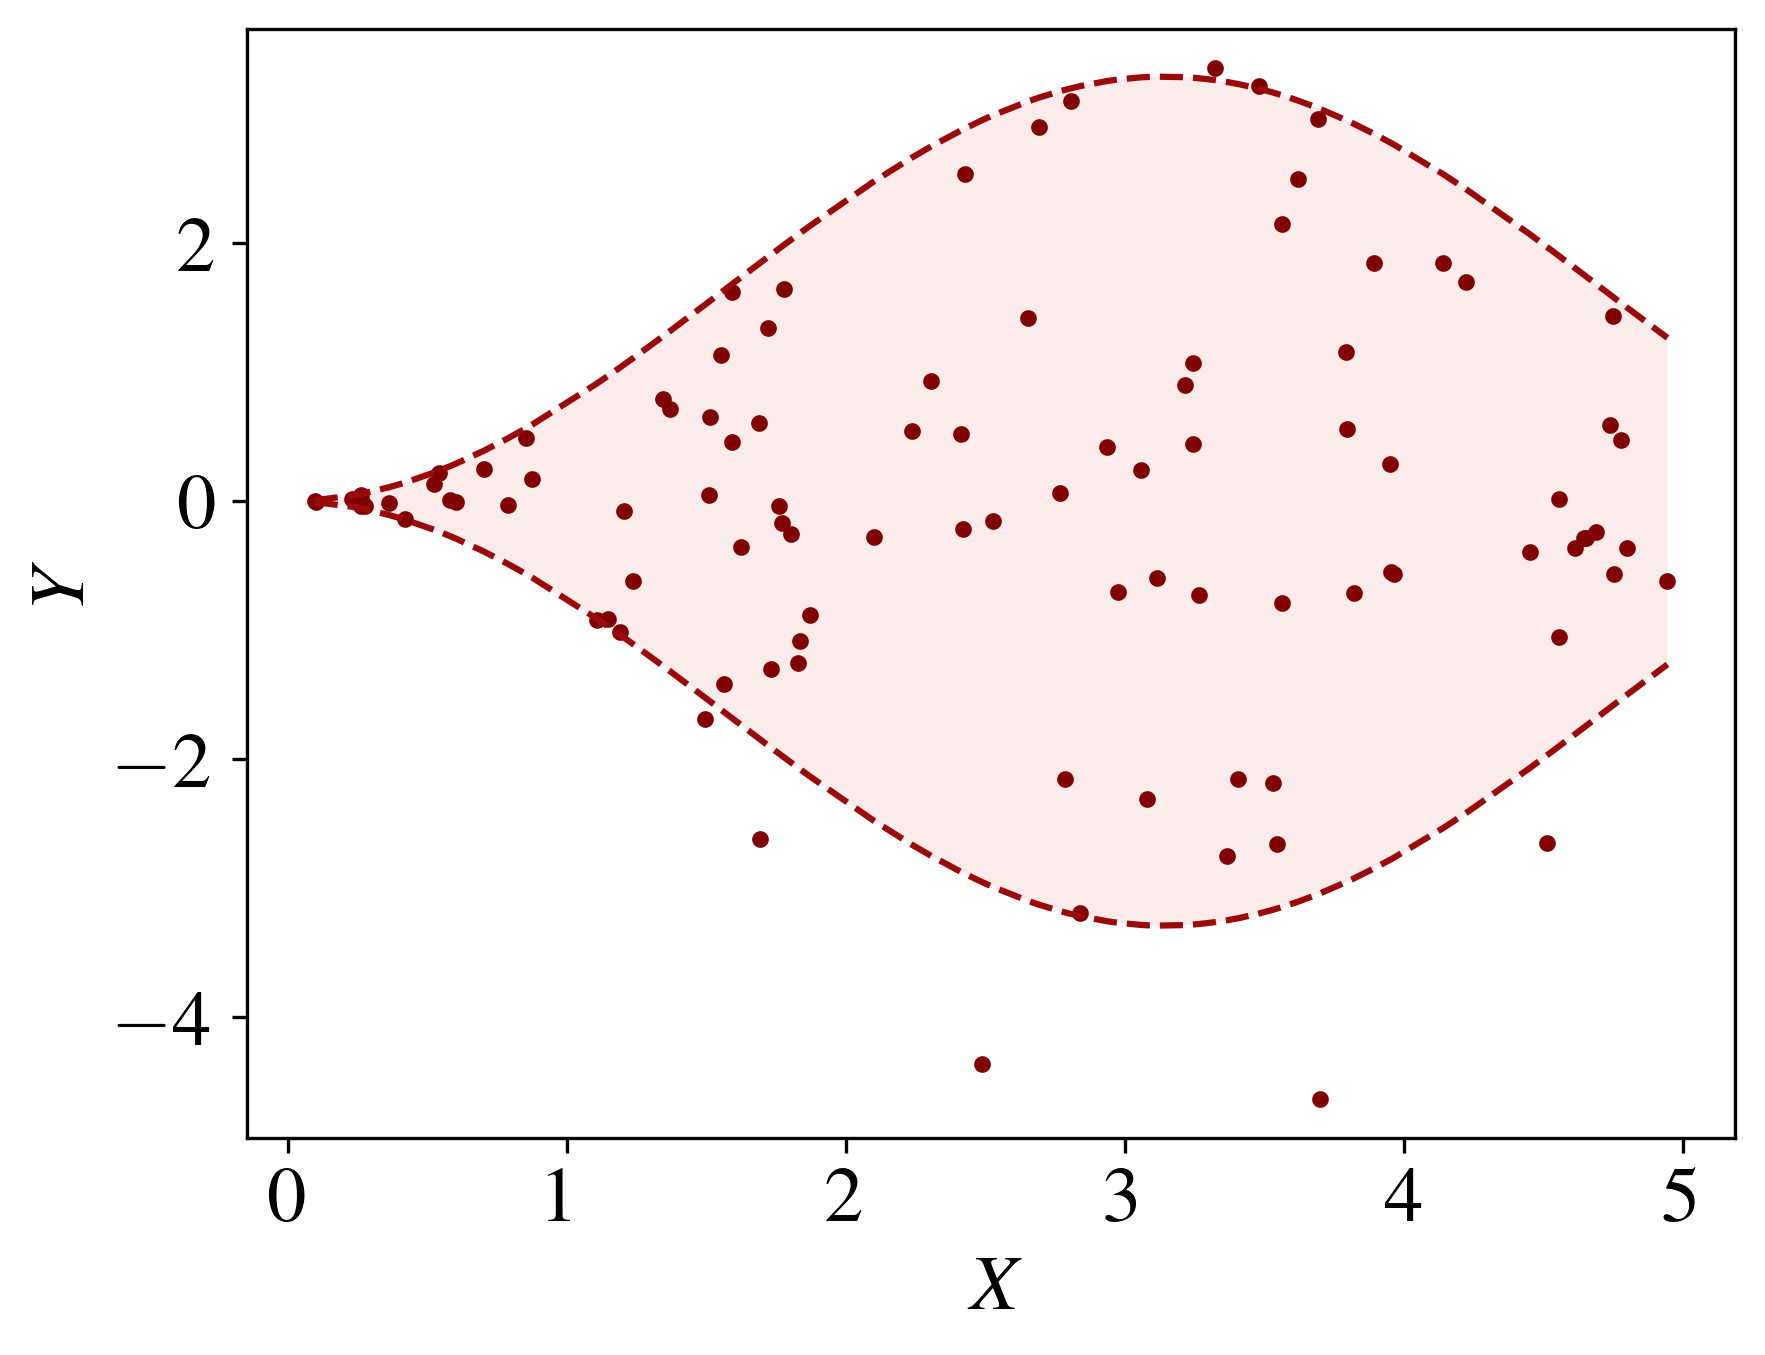
\includegraphics[width=\textwidth, height=0.55\textwidth]{Figures/coverage/conditional-coverage.png}
            \caption{Conditional cov.}
            \label{fig:coverage:cond-cover}
        \end{subfigure}
        % \vspace{-3mm}
        \caption{Different types of coverage. % Plots based in \cite{cptuto}.
        }
        \label{fig:coverage}
    \end{figure}
    \end{itemize}
\end{frame}

% \begin{frame}{Motivation}
%     \begin{itemize}%[<+->]
%         \item Let $(X, Y)\in \R^d\times\R$ be random variables: from which $n$ samples $(X_i, Y_i)_{i=1}^{n}$ are obtained.
%         \item Neither $X$ \& $Y$ marginal nor joint distributions known.
%         \item<2-> Given a new sample $X_{n+1}$ and a miscoverage level $\a\in\left[ 0, 1\right]$, we would like to: 
%         \begin{itemize}%[<+->][<+->]  
%             \item \textbf{Estimate} a predictive \textbf{interval} $\Ca$ such that the probability of $Y_{n+1}$ falling into $\Ca$ is at least $1-\a$, \textit{i.e.}
%             \begin{equation*}
%                 \P \{ Y_{n+1} \in \Ca\left(X_{n+1}\right) \} \geq 1 - \a
%             \end{equation*}
%             \item The interval to be as \textbf{small} as possible while \textbf{keeping coverage} (to be \textbf{informative}).
%             \item \textbf{Ideally}, we would like \textbf{conditional coverage}.
%         \end{itemize} 
%     \end{itemize}
% \end{frame}

% % APPROACHES TO UQ %

% \begin{frame}{Approaches}
%     % %%%%% FIGURE %%%%% %
%     \begin{figure}[ht]
%     \centering
%     \begin{subfigure}[b]{0.3\textwidth}
%         \centering
%         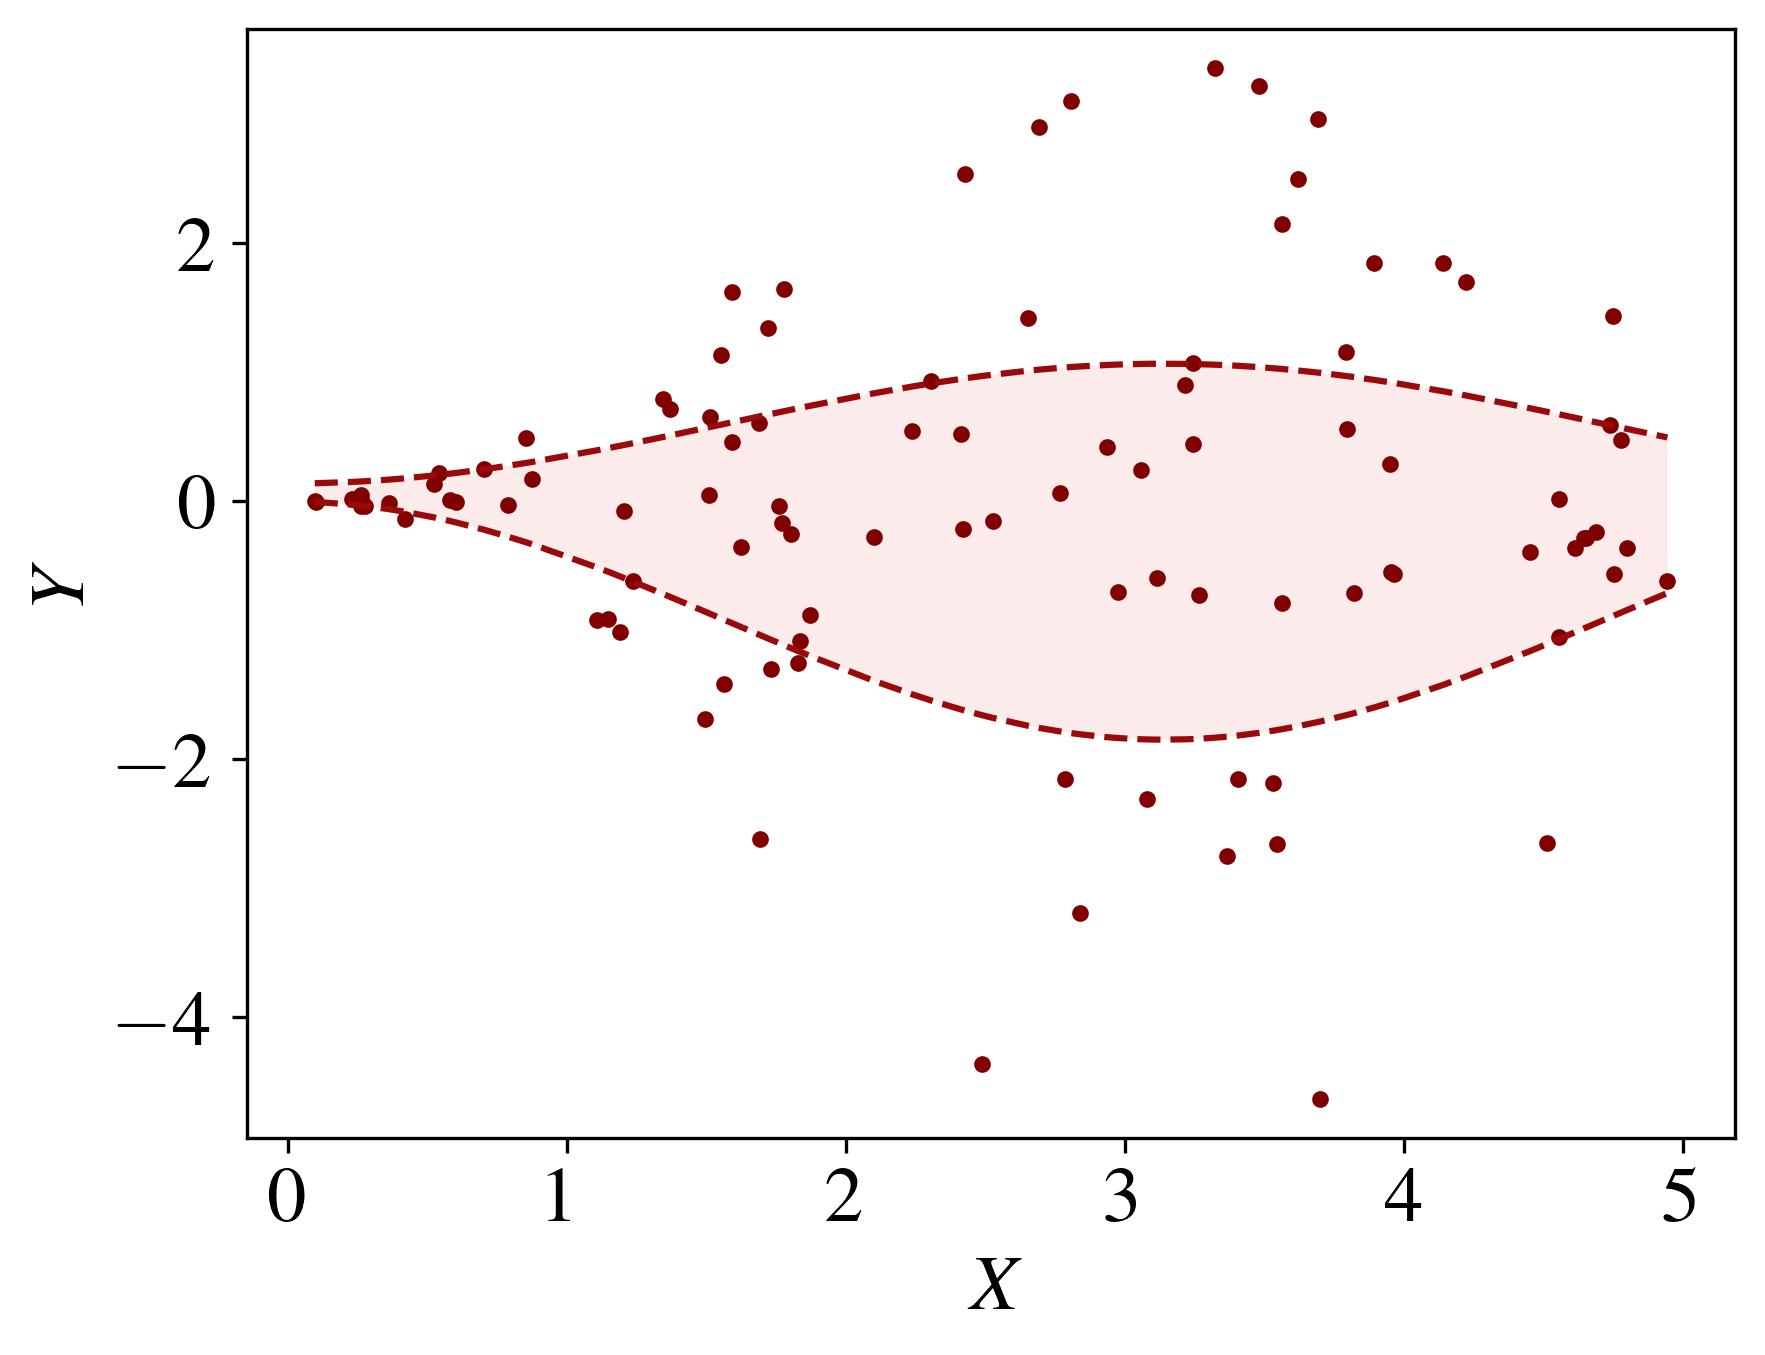
\includegraphics[width=\textwidth, height=0.55\textwidth]{Figures/coverage/no-coverage.png}
%         \caption{No coverage}
%         \label{fig:coverage:no-cover}
%     \end{subfigure}
%     \hfill
%     \begin{subfigure}[b]{0.3\textwidth}
%         \centering
%         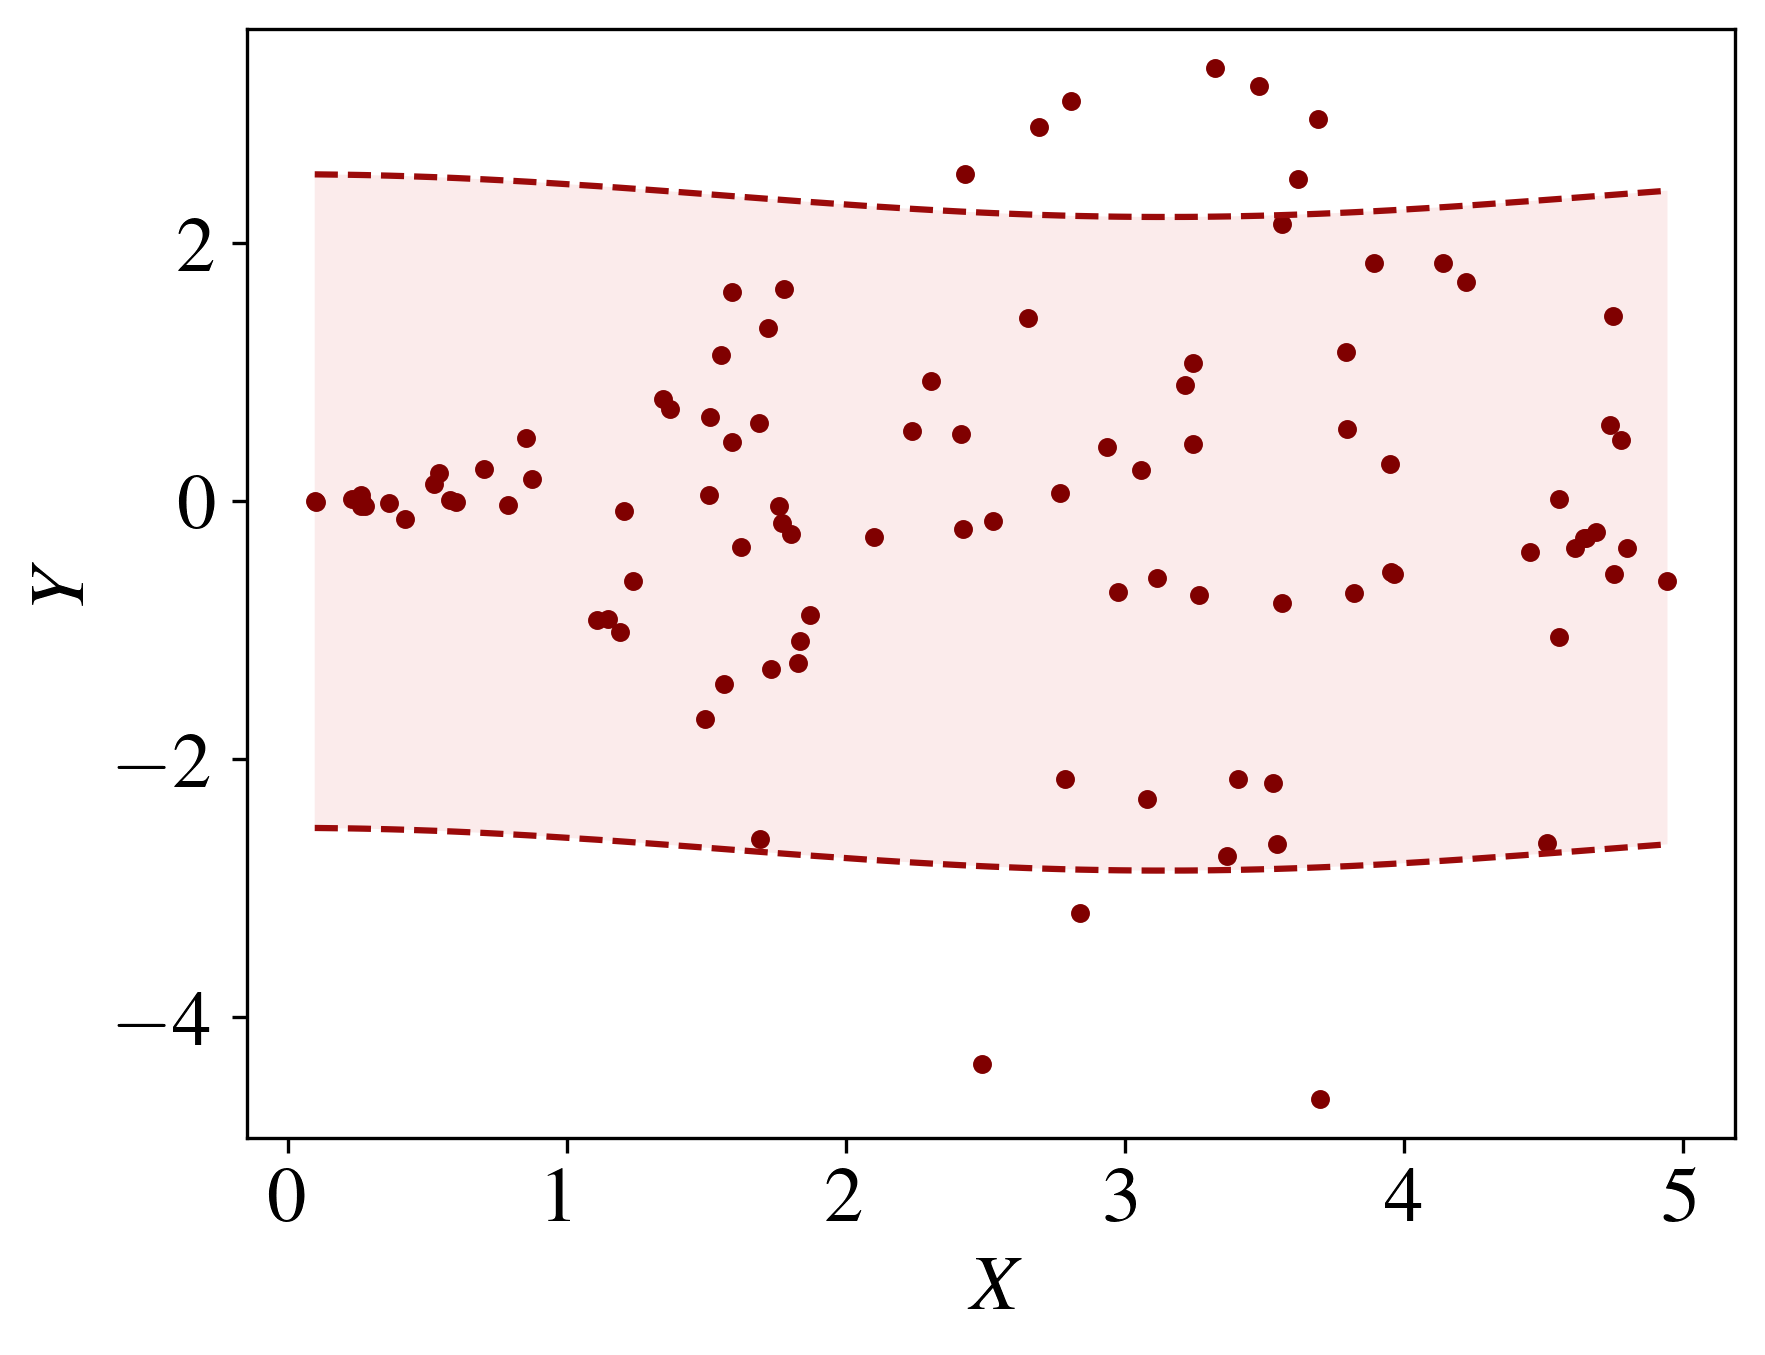
\includegraphics[width=\textwidth, height=0.55\textwidth]{Figures/coverage/marginal-coverage.png}
%         \caption{Marginal coverage}
%         \label{fig:coverage:marg-cover}
%     \end{subfigure}
%     \hfill
%     \begin{subfigure}[b]{0.3\textwidth}
%         \centering
%         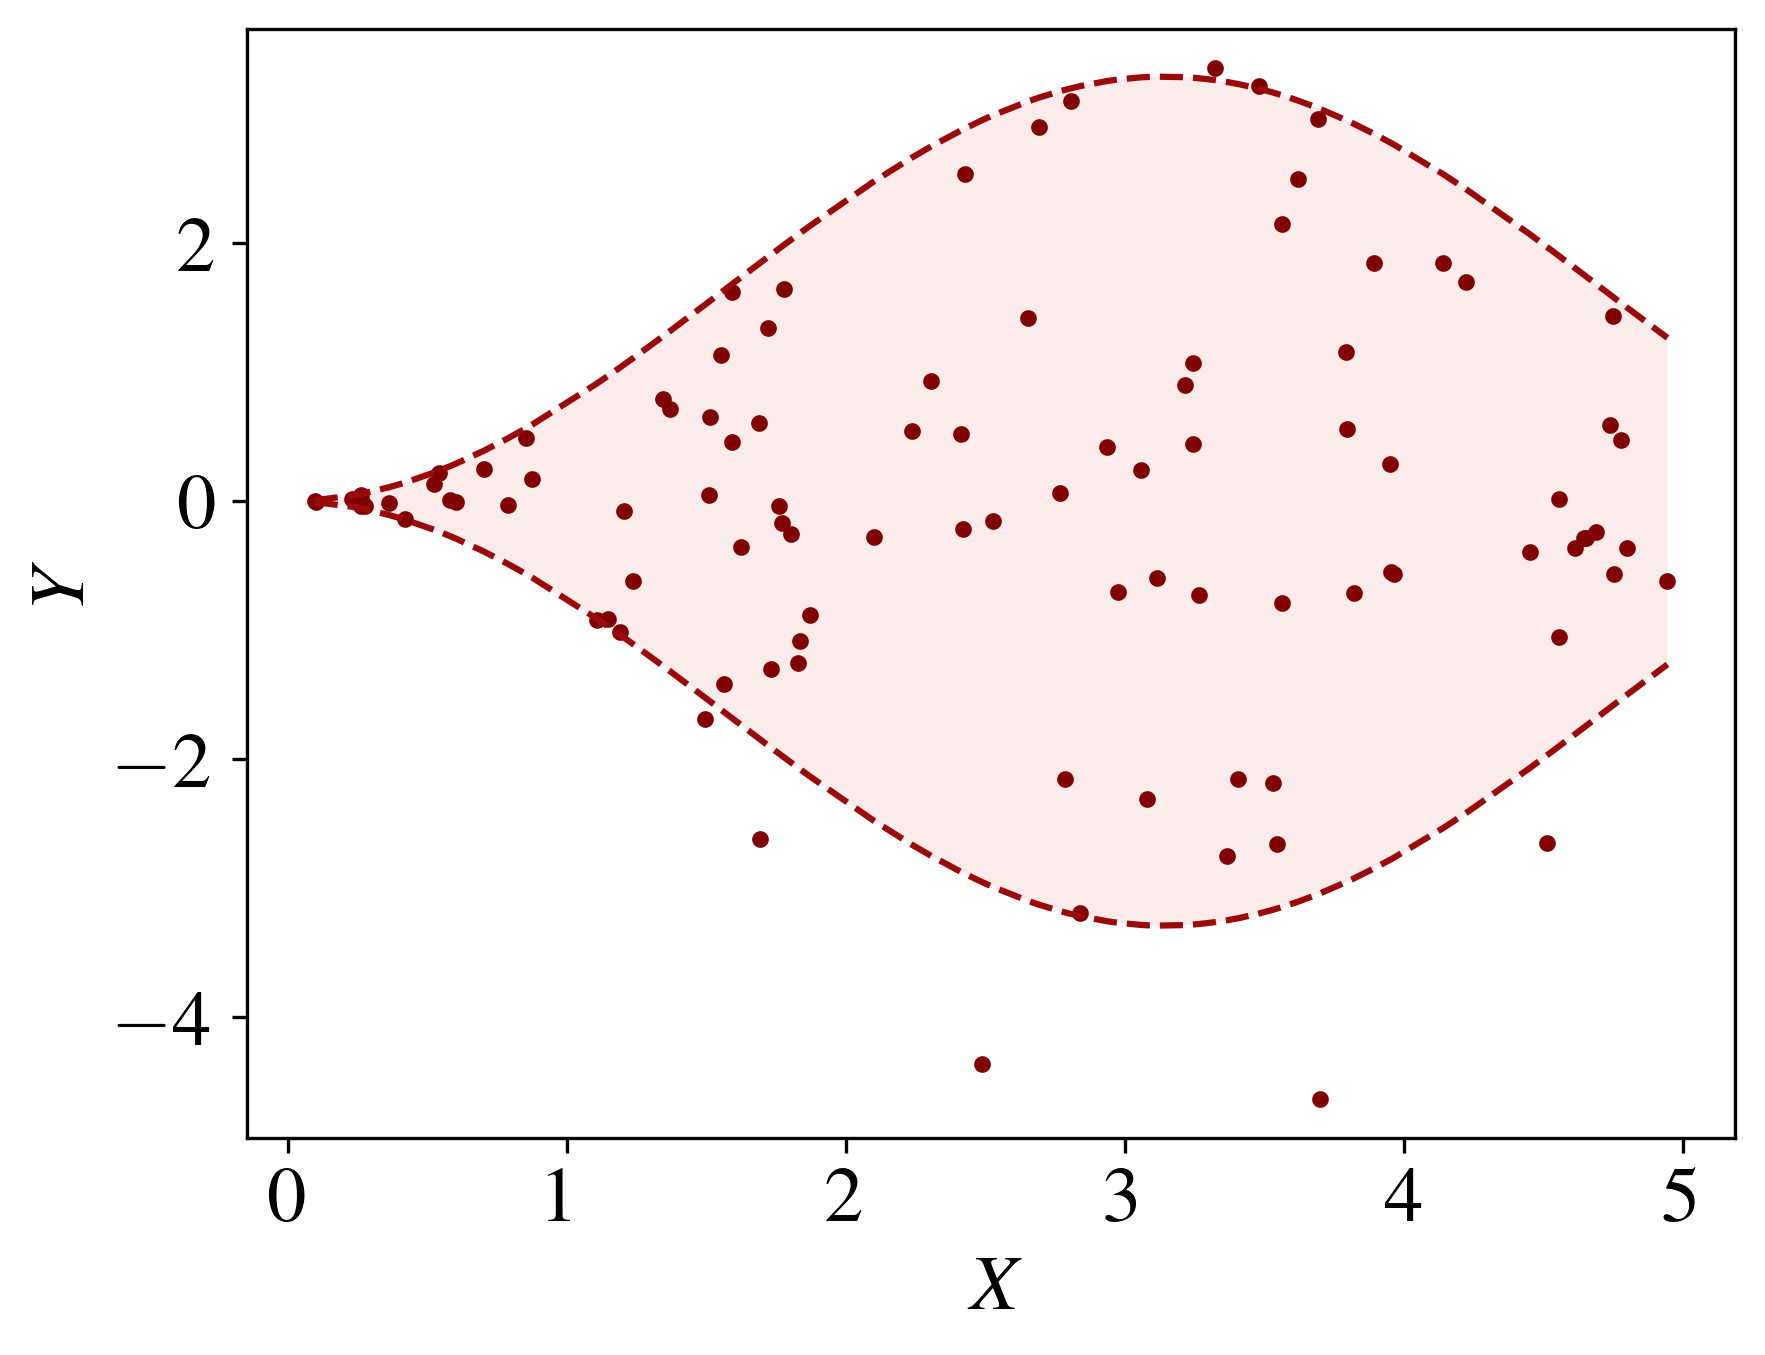
\includegraphics[width=\textwidth, height=0.55\textwidth]{Figures/coverage/conditional-coverage.png}
%         \caption{Conditional cov.}
%         \label{fig:coverage:cond-cover}
%     \end{subfigure}
%     \caption{Different types of coverage. Plots based in \cite{cptuto}.}
%     \label{fig:coverage}
% \end{figure}
% %%%%% FIGURE %%%%% %
% \vspace{-7mm}
% \begin{itemize}%[<+->][<+->]
%         \item[]
%         \item<2-> \textbf{Quantile regression} (QR):
%             \begin{enumerate}
%                 \item Fit 2 estimators $\Hat{\mu}_{\frac{\a}{2}}$, $\Hat{\mu}_{1 - \frac{\a}{2}}$ for quantiles $\frac{\a}{2}$ \& $1-\frac{\a}{2}$
%                 \item For a new sample $X_{n+1}$, prescribe: 
%                 \vspace{-3mm}
%                 $$ \Ca(X_{n+1}) = \left[ \Hat{\mu}_{\frac{\a}{2}}\left(X_{n+1}\right),\ \Hat{\mu}_{1-\frac{\a}{2}}\left(X_{n+1}\right) \right]\ $$
%             \end{enumerate}
%         \vspace{-3mm}
%         \item<2-> $\mu_{\frac{\a}{2}}$ \& $\mu_{1-\frac{\a}{2}}$ trained with all data $\{(X_i,Y_i)_{i=1}^n\}$ $\Longrightarrow$ $\Ca$ may be under/over-confident out of training $\Longrightarrow$ no valid coverage sought \xmark
        % $\Large\color{\green}{\checkmark}$
%     \end{itemize}
% \end{frame}

%%% Conformal prediction %%% (4 pp)

\section{Conformal prediction}

% SCP %

\begin{frame}{Split Conformal Prediction (SCP)}
    We need to use out-of-training data to understand how errors distribute: we need to "\textit{conformalize}" the predictions to the data using a "\textit{conformity score}". SCP proposes:
    \begin{enumerate}
        \item Split data into \textbf{training} $\mathrm{Tr}$ \& \textbf{calibration} $\mathrm{Cal}$.
        \item Obtain $\Hat{\mu}$ by training it in $\mathrm{Tr}$.
        \item Obtain a set $\S$ of conformity scores by using the $\mathrm{Cal}$ set: $\S_{\rm{Cal}}:=\{ \left|Y_i - \Hat{\mu}(X_i)\right|, i\in \mathrm{Cal}\}$.
        \item \only<1>{Compute the $1-\a$ "\textit{empirical quantile}" of $\S_{\rm{Cal}}$: $q_{1-\a}(\S_{\rm{Cal}})$.} \only<2->{Compute $(1-\a)\left(\frac{1}{\#\mathrm{Cal}}+1\right)$ quantile of $\S_{\rm{Cal}}$: $q_{1-\a}(\S_{\rm{Cal}})$.} \pause % the pause effect allows to create a "5th slide" without jumping to the 5th item (which will now be placed to the 6th slide)
        \item<3-> For a new sample $X_{n+1}$, return 
        \begin{equation*}
            \label{eq:scp}
            \Hat{\Ca} = \left[\Hat{\mu}(X_{n+1}) - q_{1-\a}(\S_{\rm{Cal}}),\ \Hat{\mu}(X_{n+1}) + q_{1-\a}(\S_{\rm{Cal}})\right]
        \end{equation*}
        \item[]<3-> \vspace{-2mm}
        \begin{tcolorbox}[colback=red!5,colframe=red!40!black,title=Note]
            The only hypothesis required is \textbf{data exchangeability}.
        \end{tcolorbox}
    \end{enumerate}
\end{frame}

% CQR (overlapping SCP)

\begin{frame}{Conformalized Quantile Regression (CQR)}
    We need to use out-of-training data to understand how errors distribute: we need to "\textit{conformalize}" the predictions to the data using a "\textit{conformity score}". \cancel{SCP} \textcolor{red}{CQR} proposes:
    \begin{enumerate}
        \item Split data into \textbf{training} $\mathrm{Tr}$ \& \textbf{calibration} $\mathrm{Cal}$.
        \item Obtain \cancel{$\Hat{\mu}$} \textcolor{red}{$\hat{\mu}_{\mathrm{down}}$ \& $\hat{\mu}_{\mathrm{up}}$} trained in $\mathrm{Tr}$.
        \item Obtain a set $\S$ of conformity scores by using the $\mathrm{Cal}$ set: \textcolor{red}{$\S_{\rm{Cal}}:=\{ \mathrm{max}\left(\hat{\mu}_{\mathrm{down}}(X_i) - Y_i,\ Y_i - \hat{\mu}_{\mathrm{up}}(X_i)\right), i\in \mathrm{Cal}\}$}.
        \item Compute $(1-\a)\left(\frac{1}{\#\mathrm{Cal}}+1\right)$ quantile of $\S_{\rm{Cal}}$: $q_{1-\a}(\S_{\rm{Cal}})$.
        \item For a new sample $X_{n+1}$, return 
        \textcolor{red}{\begin{equation*}
            \label{eq:cqr}
            \hspace{-5mm}
            \Hat{\Ca}(X_{n+1}) = \left[\hat{\mu}_{\mathrm{down}}(X_{n+1}) - q_{1-\a}\left(\S_{\mathrm{Cal}}\right),\ \hat{\mu}_{\mathrm{up}}(X_{n+1}) + q_{1-\a}\left(\S_{\mathrm{Cal}}\right)\right]
        \end{equation*}}
        \item[] \vspace{-6mm}
        \begin{tcolorbox}[colback=red!5,colframe=red!40!black,title=Note]
            The only hypothesis required is \textbf{data exchangeability}.
        \end{tcolorbox}
    \end{enumerate}
\end{frame}

% FCP %

% \begin{frame}{Full Conformal Prediction (FCP)}
%     SCP attains expected coverage but needs a dataset large enough for $\Ca$ to be informative. FCP proposes a workaround, its idea is:
%     \begin{enumerate}  
%         \item \textit{Discretize} target space $\mathcal{Y}$ into $N$ candidates $Y_j$.
%         \item Initialize $\Hat{\mathcal{Y}}_{\rm{low}} = \{\}$ and for $j \in \{1, \ldots, N\}$, do:
%         \begin{itemize}%[<+->][<+->]
%             \item Fit $\mu_j$ using $\rm{Tr}_j=\{\left(X_t,Y_t\right)\}^T_{t=1}\cup \{(X_{T+1}, Y_j)\}$ as training
%             \item Set $\S_j=\{ s_{\Hat{\mu}_j}(X_i, Y_i) \}_{i=1}^T\cup \{s_{\Hat{\mu}_j}(X_{T+1}, Y_j)\}$, the in-training conformity scores.
%             \item Set the $1-\a$ empirical quantile of $\S_{j}$: $q^j_{1 - \a}(\S_{j})$
%             \item If $s_{\Hat{\mu}_j}(X_{T+1}, Y_j) \leq q^j_{1 - \a}(\S_{j})$, then add $Y_j$ to $\Hat{\mathcal{Y}}_{\rm{low}}$
%         \end{itemize}
%         \item Return $\Ca(X_{T+1})=\Hat{\mathcal{Y}}_{\rm{low}}$.
%         \item[] % \vspace{-3.5mm}
%         \begin{tcolorbox}[colback=red!5,colframe=red!40!black,title=Note]
%             FCP workaround is \textbf{computationally expensive}: it proposes $N$ fits!
%         \end{tcolorbox}
%     \end{enumerate}
% \end{frame}

% Other flavours %

\begin{frame}{Other flavours}
    Then, other flavours are proposed to reconcile this trade-off between statistical and computational efficiency, for instance CV$+$ \& J$+$aB:
    \begin{figure}[ht]
        \centering
        % \includegraphics{}
        \begin{tikzpicture}
            \definecolor{tred}{HTML}{800000}
            % Draw the horizontal arrows
            \draw[thick, ->, tred] (1, 0) -- (10, 0) node[anchor=north, pos=0.5] {Statistical Efficiency};
            \draw[thick, <-, tred] (1, -0.6) -- (10, -0.6) node[anchor=north, pos=0.5] {Computational Efficiency};
            % Draw the boxes
            \draw (1, -1.8) rectangle (3.4, -1.2) node[pos=0.5] {SCP \& CQR};
            \draw (4.2, -1.8) rectangle (5.2, -1.2) node[pos=0.5] {CV+};
            \draw (6, -1.8) rectangle (8, -1.2) node[pos=0.5] {Jackknife+};
            \draw (9, -1.8) rectangle (10, -1.2) node[pos=0.5] {FCP};
            % Draw the nested conformal prediction arrow
            \draw[thick, |-|, tred] (1, -2.1) -- (8, -2.1) node[anchor=north, pos=0.5] {Nested Conformal Prediction};
        \end{tikzpicture}
        \caption{Trade-off between statistical \& computational efficiency. 
        %Based on \cite{cptuto}.
        }
        \label{fig:trade-off}
    \end{figure}
    \begin{itemize}%[<+->][<+->]
        \vspace{-3mm}
        \item Both CV$+$ \& J$+$aB are based on defining multiple folds to apply a similar methodology as SCP: cross-validation \& leave-one-out (LOO) folds, respectively.
    \end{itemize}  
\end{frame}

% % CQR %

% \begin{frame}{CQR}
%     None of former 4 methodologies yield adaptive intervals. CQR deals with this "\textit{conformalizing}" quantile regression:
%     \begin{enumerate}
%         \item Split data into \textbf{training} $\mathrm{Tr}$ \& \textbf{calibration} $\mathrm{Cal}$.
%         \item Obtain $\hat{\mu}_{\mathrm{down}}$ for the lower quantile and $\hat{\mu}_{\mathrm{up}}$ for the upper training with $\mathrm{Tr}$.
%         \item Define the set $\S$ of conformity scores with $\mathrm{Cal}$ set: $\S_{\rm{Cal}}:=\{ \mathrm{max}\left(\hat{\mu}_{\mathrm{down}}(X_i) - Y_i,\ Y_i - \hat{\mu}_{\mathrm{up}}(X_i)\right), i\in \mathrm{Cal}\}$.
%         \item Compute $1-\a$ empirical quantile of $\S_{\rm{Cal}}$: $q_{1-\a}(\S_{\rm{Cal}})$.
%         \item For a new sample $X_{n+1}$, return 
        % \hspace{-10mm}
        % \begin{equation*}
        %     \label{eq:cqr}
        %     \hspace{-5mm}
        %     %\Hat{\Ca}(X_{n+1}) = \left[\hat{\mu}_{\mathrm{down}}(X_{n+1}) \pm q_{1-\a}\left(\S_{\mathrm{Cal}}\right)
        %     \Hat{\Ca}(X_{n+1}) = \left[\hat{\mu}_{\mathrm{down}}(X_{n+1}) - q_{1-\a}\left(\S_{\mathrm{Cal}}\right),\ \hat{\mu}_{\mathrm{up}}(X_{n+1}) + q_{1-\a}\left(\S_{\mathrm{Cal}}\right)\right]
        % \end{equation*}
        % \item[] \vspace{-4mm}
        % \begin{tcolorbox}[colback=red!5,colframe=red!40!black,title=Note]
        %     The only hypothesis required is \textbf{data exchangeability}.
        % \end{tcolorbox}
%     \end{enumerate}
% \end{frame}

%%% Beyond exchangeability %%% (4pp)

\section{Beyond exchangeability}

% Covariate shift %

\begin{frame}{Covariate shift: changes in features’ distribution}
    \begin{itemize}%[<+->]
        \item $\{\left(X_i, Y_i\right)\}_{i=1}^n \overset{\mathrm{exch.}}{\sim} P_X\times P_{Y|X}$
        \item $\left(X_{n+1}, Y_{n+1}\right) \sim \Tilde{P}_X\times P_{Y|X}$
        \item \textit{Tibshirani et al. (2019)} %\cite{tibshirani}'s 
        heuristic idea:
        \begin{enumerate}  
            \item Estimate how "close" a sample $X_i$ ($\sim P_X$) is \textit{w.r.t.} to the test point ($\sim \Tilde{P}_X$) using the likelihood ratio: $w(X_i):= \frac{d\Tilde{P}_X(X_i)}{dP_X(X_i)}$.
            \item Normalize the weights: $\omega_i:=\frac{w(X_i)}{\sum_{j=1}^{n+1} w(X_j)}$. 
            \item Build the predictive interval $\Ca$ using the weighted calibration samples:
            \begin{equation*}\label{eq:cp-covariate}
                \Hat{\Ca}\left(X_{n+1}\right) = \{ Y: \ s_{\Hat{\mu}}\left(X_{n+1}, Y\right) \leq q_{1-\a}\left(\{\omega_i S_i\}_{i\in\rm{Cal}}\right)  \}
            \end{equation*}
        \end{enumerate}
    \end{itemize}
    
\end{frame}

% Label shift %

\begin{frame}{Label shift: changes in target’s distribution}
    \begin{itemize}%[<+->]
        \item $\{\left(X_i, Y_i\right)\}_{i=1}^n \overset{\mathrm{exch.}}{\sim} P_{X|Y}\times P_{Y}$
        \item $\left(X_{n+1}, Y_{n+1}\right) \sim P_{X|Y}\times \Tilde{P}_{Y}$
        \item \textit{A. Podkopaev \& A. Ramdas (2021)} %\cite{podkopaev} 
        adapts former idea letting weights as function of $Y$, $\omega_i^Y$:
        \begin{enumerate}  
            \item Estimate how "close" a label $Y_i$ ($\sim P_Y$) is \textit{w.r.t.} to the hypothetical point ($\sim \Tilde{P}_Y$) using the likelihood ratio: $w(Y_i):= \frac{d\Tilde{P}_Y(Y_i)}{dP_Y(Y_i)}$.
            \item Normalize the weights: $\omega_i^Y:=\frac{w(Y_i)}{\sum_{j=1}^{n} w(Y_j) + w(Y)}$. 
            \item Build the predictive interval $\Ca$ traversing all the variable output's space and using the weighted calibration samples:
            \begin{equation*}\label{eq:cp-label}
                \Hat{\Ca}\left(X_{n+1}\right) = \{ Y: \ s_{\Hat{\mu}}\left(X_{n+1}, Y\right) \leq q_{1-\a}\left(\{\omega^Y_i S_i\}_{i\in\rm{Cal}}\right)  \}
            \end{equation*}
        \end{enumerate}
    \end{itemize}
\end{frame}

% EnbPI (I): idea %

\begin{frame}{Time series data: samples (temporal) auto-correlation}
\begin{itemize}%[<+->]
    \item[] 
    \begin{itemize}%[<+->][<+->]  
        \item Assume a setup like $Y_t = \mu\left(X_t\right) + \epsilon_t$, where $\epsilon_t$ are \textit{i.i.d.} according to a cumulative distribution function $F$. 
        \item Let the first $T$ sample points $\mathcal{D}:=\{\left(X_t, Y_t\right)_{t=1}^T\}$ be training data: we \textbf{want} a \textbf{sequence} of $s\geq 1$ \textbf{intervals} of $\a$ miscoverage level, $\{\mathcal{C}^\alpha_{T,T+i}\}_{i=1}^s$ (for the unknown labels $\{{Y}^\alpha_{T+i}\}_{i=1}^s$).
        \begin{itemize}%[<+->]
            \item $s$ is the batch size (nº steps to look ahead)
        \end{itemize}
        \item Also, once \textbf{new samples} $\{\left(X_{T+i}, Y_{T+i}\right)\}_{i=1}^s$ become \textbf{available}, we would like to also \textbf{leverage them}.
        \begin{itemize}%[<+->]
            \item We want to use the most recent $T+s$ points for the $\{\mathcal{C}^\alpha_{T+s,j}\}_{j=T+s+1}^{=T+2s}$ intervals.
        \end{itemize}
    \end{itemize}
    \item[]<2-> $\Longrightarrow$ \textit{C. Xu \& Y. Xie (2021)} %\cite{chenxu2021a} 
    proposes the "\textit{EnbPI}" methodology: 
    \begin{itemize}%[<+->]
        \item It uses no data-splitting but LOO estimators ($\Hat{\mu}_{-i}$ model trained with $\mathcal{D}\setminus \{(X_i, Y_i)\}$).
        \item Models not refitted during test time, but newest samples' residuals used to further \textit{conformalize} predictions.
    \end{itemize}
        
\end{itemize}
\end{frame}

% EnbPI (II): guarantees %

\begin{frame}{EnbPI idea}
    There are $T$ training samples and we build $T_1$ intervals (indices $T+1, \ldots, T+T_1$):
    \begin{itemize}%[<+->][<+->]
        \item Obtain $B$ bootstrapped models $\mu^b$ by:
        \begin{itemize}%[<+->]
            \item Sampling, with replacement, an index set $S_b:=\left(i_1,\ldots, i_T\right)$ % from indices $(1,\ldots,T)$.
            \item Fitting the bootstrapped model with $S_b$ % : $$\hat{\mu}^b(\cdot) \leftarrow \mathcal{A}\left(\left\{\left(X_i,Y_i\right), i \in S_b\right\}\right)\ .$$
        \end{itemize}
        \item For $i=1, \ldots, T$:  % we create an ensemble model with the bootstrapped's by agreggating them (to avoid overfitting)
        \begin{itemize}%[<+->]
            \item Aggregate $\mu^b$ with any function $\phi$: obtaining $\Hat{\mu}^\phi_{-i}$. 
            \item Compute conformity scores: $\epsilon_i^{\phi}:=\left|Y_i-\Hat{\mu}^\phi_{-i}(X_i)\right|$.
        \end{itemize}
        \item For each $t=T+1,\ldots, T+T_1$ timestamps, return in batches of $s$ size: $$
        \hspace{-15mm}
        \Hat{\mathcal{C}}_{T, t}^{\alpha}\left(X_t\right) = % \left[\Hat{\mu}^\phi_{-t}(X_t) - w_t^\phi,\ \Hat{\mu}^\phi_{-t}(X_t) + w_t^\phi \right],
        \left[\Hat{\mu}^\phi_{-t}(X_t) \pm w_t^\phi\right], \mathrm{where}\ 
        \begin{cases}
            \Hat{\mu}^\phi_{-t}(X_t):\ 1-\a\ \mathrm{quant.}\ \{\Hat{\mu}^\phi_{-i}(X_t)\}_{i=1}^T\\
            w_t^\phi:\ 1-\a\ \mathrm{quantile}\ \mathrm{of}\ \{\epsilon^\phi_{i}\}_{i=1}^T
        \end{cases}
        $$
        \item "\textit{Partial fit}" \textbf{step}: for each $s$ returned intervals, conformity score $w^\phi_t$ is re-computed with the most recent observations. 
    \end{itemize}
    
\end{frame}

%%% Results %%% (8pp)

\section{Results}

%% Assessment %% (1p)

\subsection{Assessment}

\begin{frame}{Metrics definition}
The following metrics will be used:
\begin{itemize}%[<+->][<+->]
    \item \textbf{Coverage level}: \textit{i.e.} fraction of true labels lying within the prediction intervals (the closer to $1-\a$, the better)
    \item \textbf{Interval width}: intervals' mean width (the smaller, the better)
    \item \textbf{"\textit{Informativeness}"}: best width-coverage ratio, assessed through CWC score (the higher, the better):
    \vspace{-3mm}
        $$ \hspace{-10mm} \mathrm{CWC} = (1 - w) * \exp{\left(-\eta (c - (1-\alpha))^2\right)},\ \mathrm{with}\ 
        \begin{cases}
            w\ \mathrm{mean}\ \mathrm{width}\\
            c\ \mathrm{attained}\ \mathrm{coverage}\\
            \eta\ \mathrm{balancing}\ \mathrm{term}
        \end{cases}$$ 
    \vspace{-2mm}
    \item \textbf{Adaptability}: ability of achieving conditional coverage, assessed through SSC score (the closer to $1-\a$, the better).
    \begin{itemize}%[<+->]
        \item Maximum coverage violation along all width groups.
        \item Only usable for non-constant width intervals.
    \end{itemize}
    % \vspace{-5mm}
    \item \textbf{Computational efficiency}: measured by CPU time.

\end{itemize}
\end{frame}

%% Regression problem %% (2pp)

\subsection{Regression problem}

% Dataset %

\begin{frame}{Data \& modeling}
\begin{columns} % the "c" option specifies center vertical alignment
        \vspace{-5mm}
        \begin{column}{0.5\textwidth} % adjust the column width to suit your needs
            A tabular regression problem is considered with:
            \begin{itemize}%[<+->][<+->]
                \item The \texttt{sklearn} built-in \href{https://scikit-learn.org/stable/modules/generated/sklearn.datasets.fetch_california_housing.html}{California Housing dataset} ($20,640$ samples, 8 features).
                \item A (light) gradient boosting regressor, \texttt{LGBM}, automatically fine-tuned through grid-search. 
                \item A 5-fold cross-validation assessment for $\a=0.20$ miscoverage level.
            \end{itemize}
        \end{column}
        \begin{column}{0.5\textwidth} % adjust the column width to suit your needs
            % \textbf{Figure Column:}
            \begin{figure}
                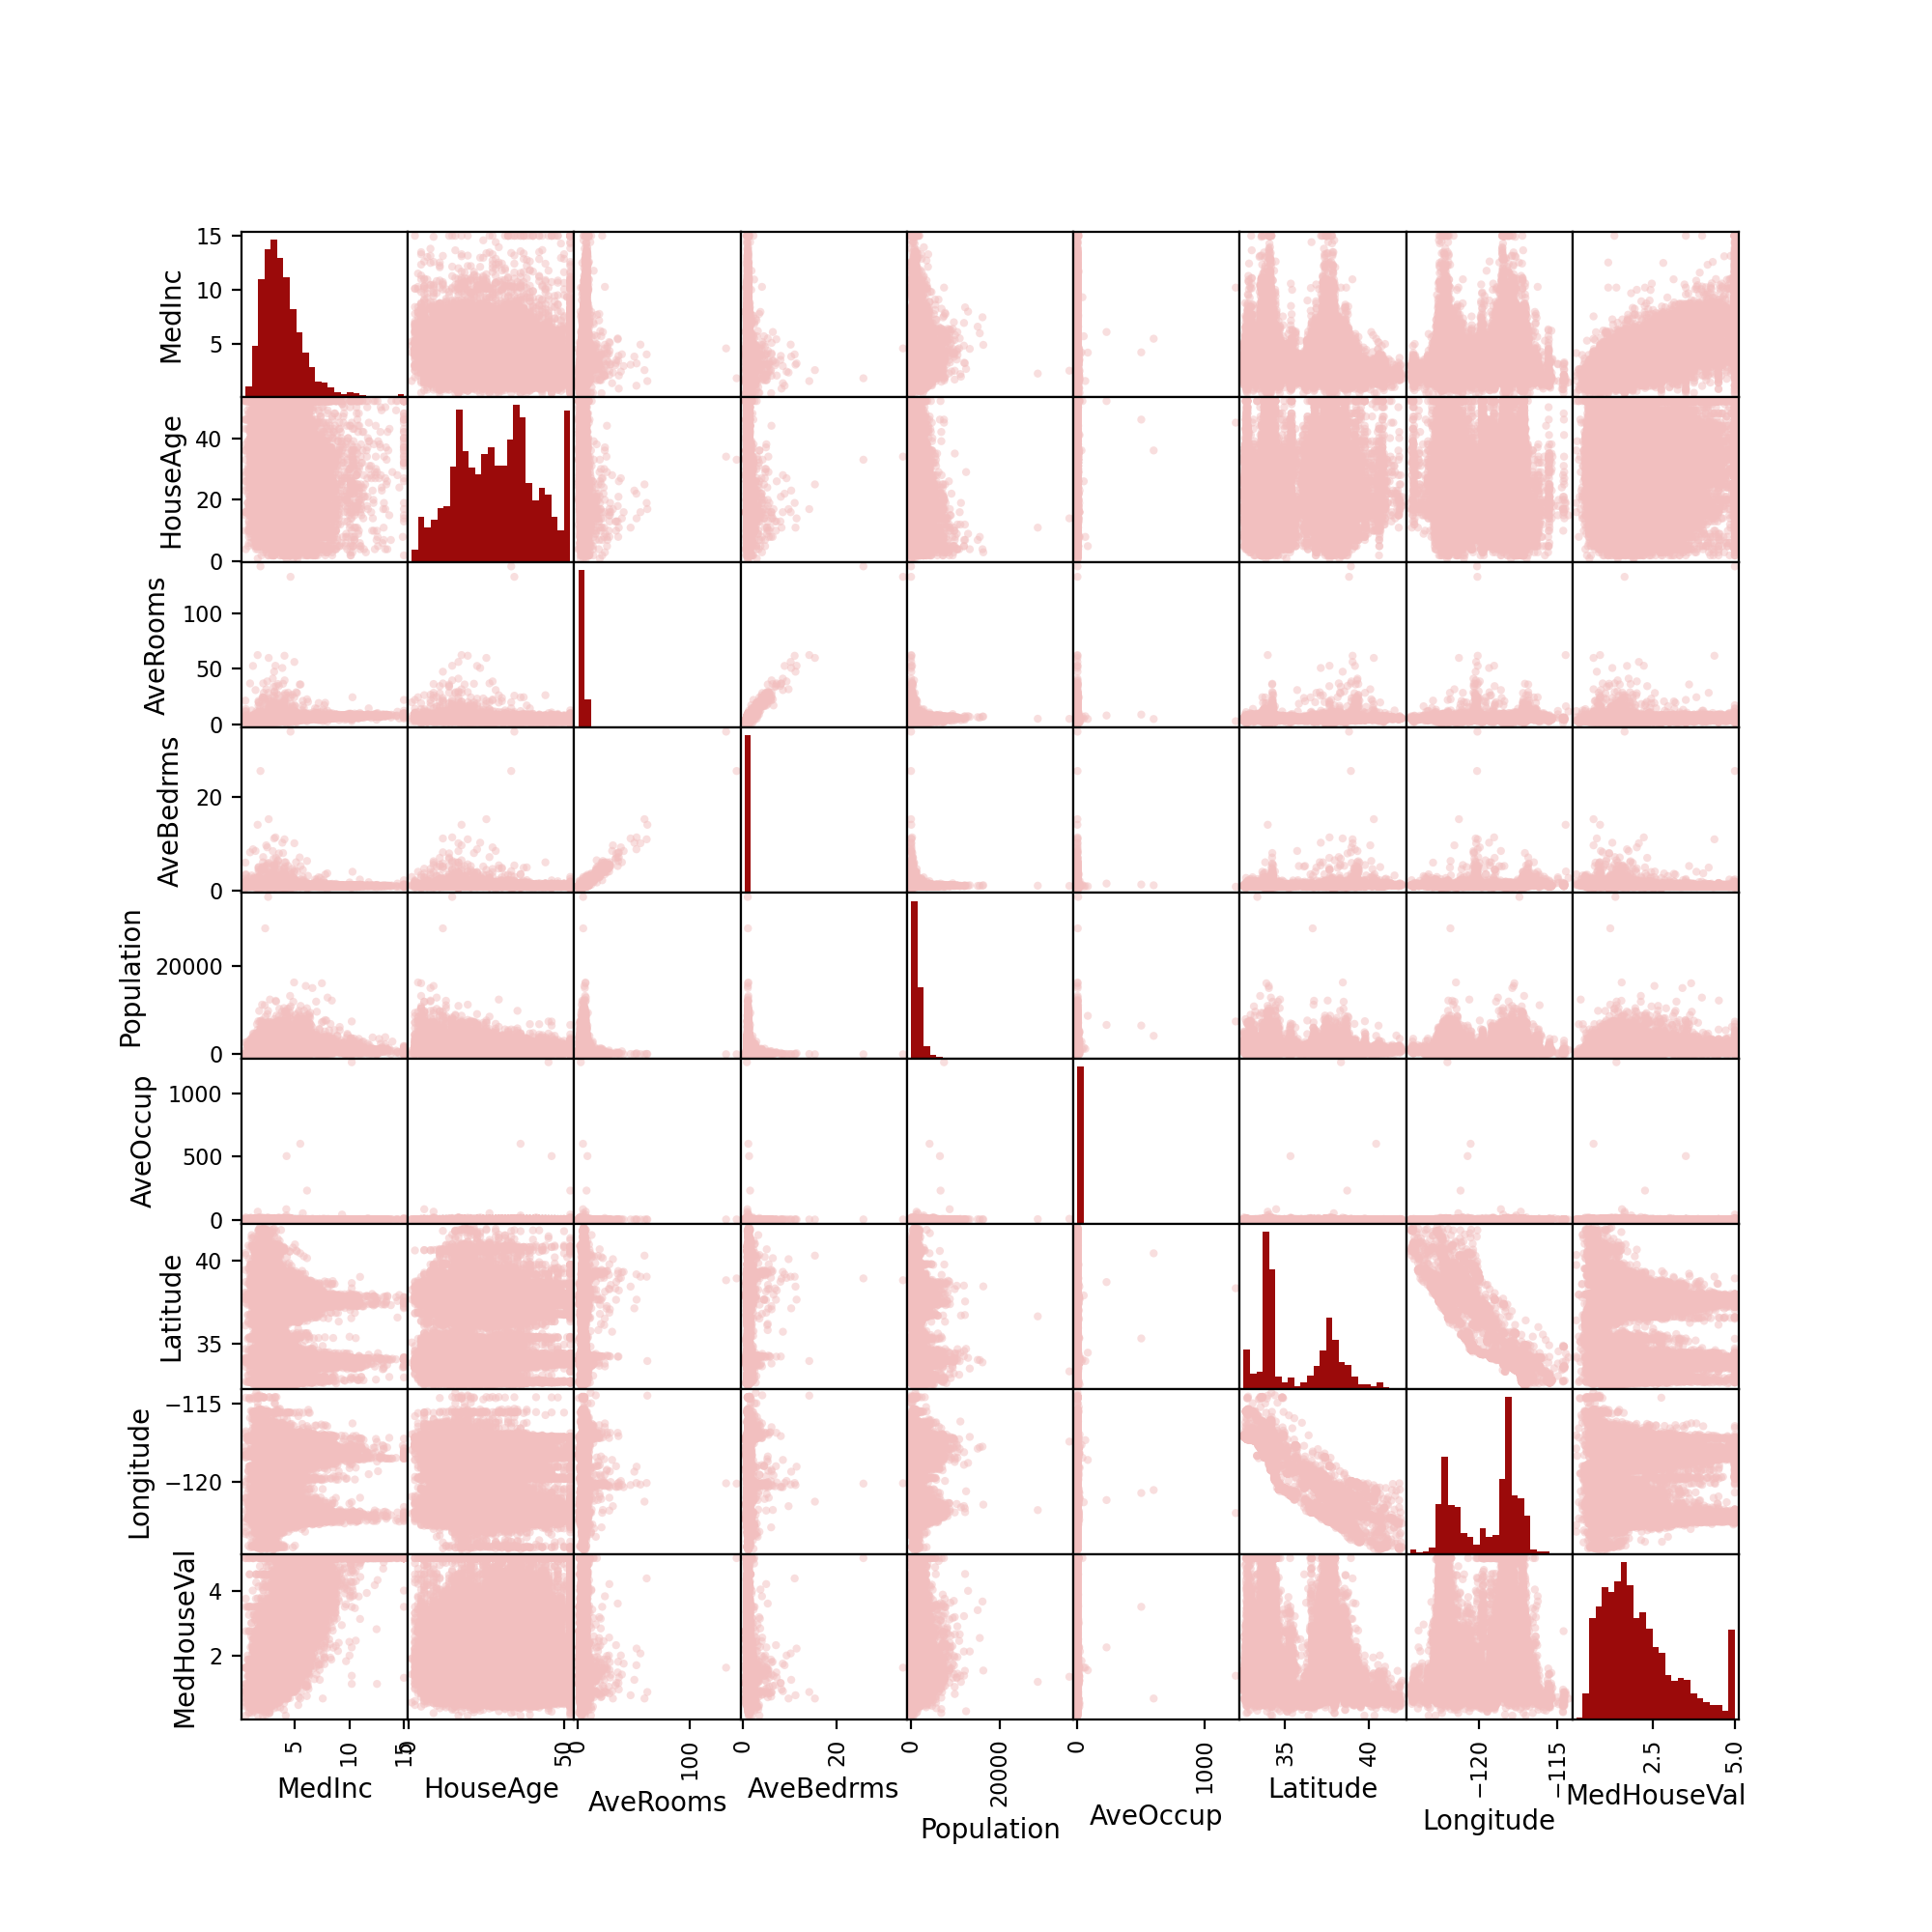
\includegraphics[width=\textwidth]{Figures/regression/data-regression-problem.png}
                \caption{Marginal distributions.}
            \end{figure}
        \end{column}
    \end{columns}
\end{frame}

% Metrics & visualizations %

\begin{frame}{Metrics table}

    \begin{table}[ht]
        
        \begin{subtable}{.5\textwidth}
            \hspace{-32mm}
            \begin{tabular}{|c|c|c|c|c|}
            % \hline
            \rowcolor{ColHead}\textcolor{white}{Strategy} & \textcolor{white}{Coverage} & \textcolor{white}{RMSE} & \textcolor{white}{Train. time} & \textcolor{white}{Inf. time}\\ \hline
            \cellcolor{RowHead}SCP & 0.806 $\pm$ 0.008 & 0.472 $\pm$ 0.007 & 1.6 $\pm$ 0.2 & 0.07 $\pm$ 0.05\\
            \cellcolor{RowHead}CV+ & 0.853 $\pm$ 0.004 & 0.467 $\pm$ 0.009 & 9 $\pm$ 3 & 8.0 $\pm$ 0.3\\
            \cellcolor{RowHead}J+aB & 0.734 $\pm$ 0.007 & 0.467 $\pm$ 0.009 & 51 $\pm$ 5 & 9.7 $\pm$ 0.4\\
            \cellcolor{RowHead}CQR & 0.805 $\pm$ 0.010 & 0.494 $\pm$ 0.013 & 2.6 $\pm$ 0.1 & 0.10 $\pm$ 0.04\\
            \hline
            \end{tabular}
        %\caption{Coverage, RMSE, training \& inference times.}
        %\label{subtab:regression-metrics-1}
        \end{subtable}
        
        \begin{subtable}{.5\textwidth}
            \hspace{-35mm}
            \begin{tabular}{|c|c|c|c|c|}
            \rowcolor{ColHead}\textcolor{white}{Strategy} & \textcolor{white}{Coverage} & \textcolor{white}{Width} & \textcolor{white}{CWC} & \textcolor{white}{SSC}\\ \hline
            \cellcolor{RowHead}SCP & 0.806 $\pm$ 0.008 & 0.971 $\pm$ 0.015 & 0.798 $\pm$ 0.004 & ---\\
            \cellcolor{RowHead}CV+ & 0.853 $\pm$ 0.004 & 1.042 $\pm$ 0.005 & 0.784 $\pm$ 0.002 & 0.65 $\pm$ 0.01\\
            \cellcolor{RowHead}J+aB & 0.734 $\pm$ 0.007 & 0.710 $\pm$ 0.003 & 0.853 $\pm$ 0.001 & --- % 0.39 $\pm$ 0.02
            \\
            \cellcolor{RowHead}CQR & 0.805 $\pm$ 0.010 & 1.013 $\pm$ 0.013 & 0.790 $\pm$ 0.004 & 0.75 $\pm$ 0.04\\
            \hline
            \end{tabular}
        %\caption{Coverage, width, coverage width-based criterion (CWC) score \& size-stratified coverage (SSC) score.}
        %\label{subtab:regression-metrics-2}
        \end{subtable}
        %\caption{Different strategies' metrics after a 5-fold cross-validation for $\a=0.2$ regression problem.}
        %\label{tab:regression-metrics}
    \end{table}
\end{frame}

% Other visualizations %

\begin{frame}{Other visualizations}
    \begin{figure}[ht]
        \centering
        %\hspace{-10mm}
        \begin{subfigure}[b]{0.32\textwidth}
            \centering
            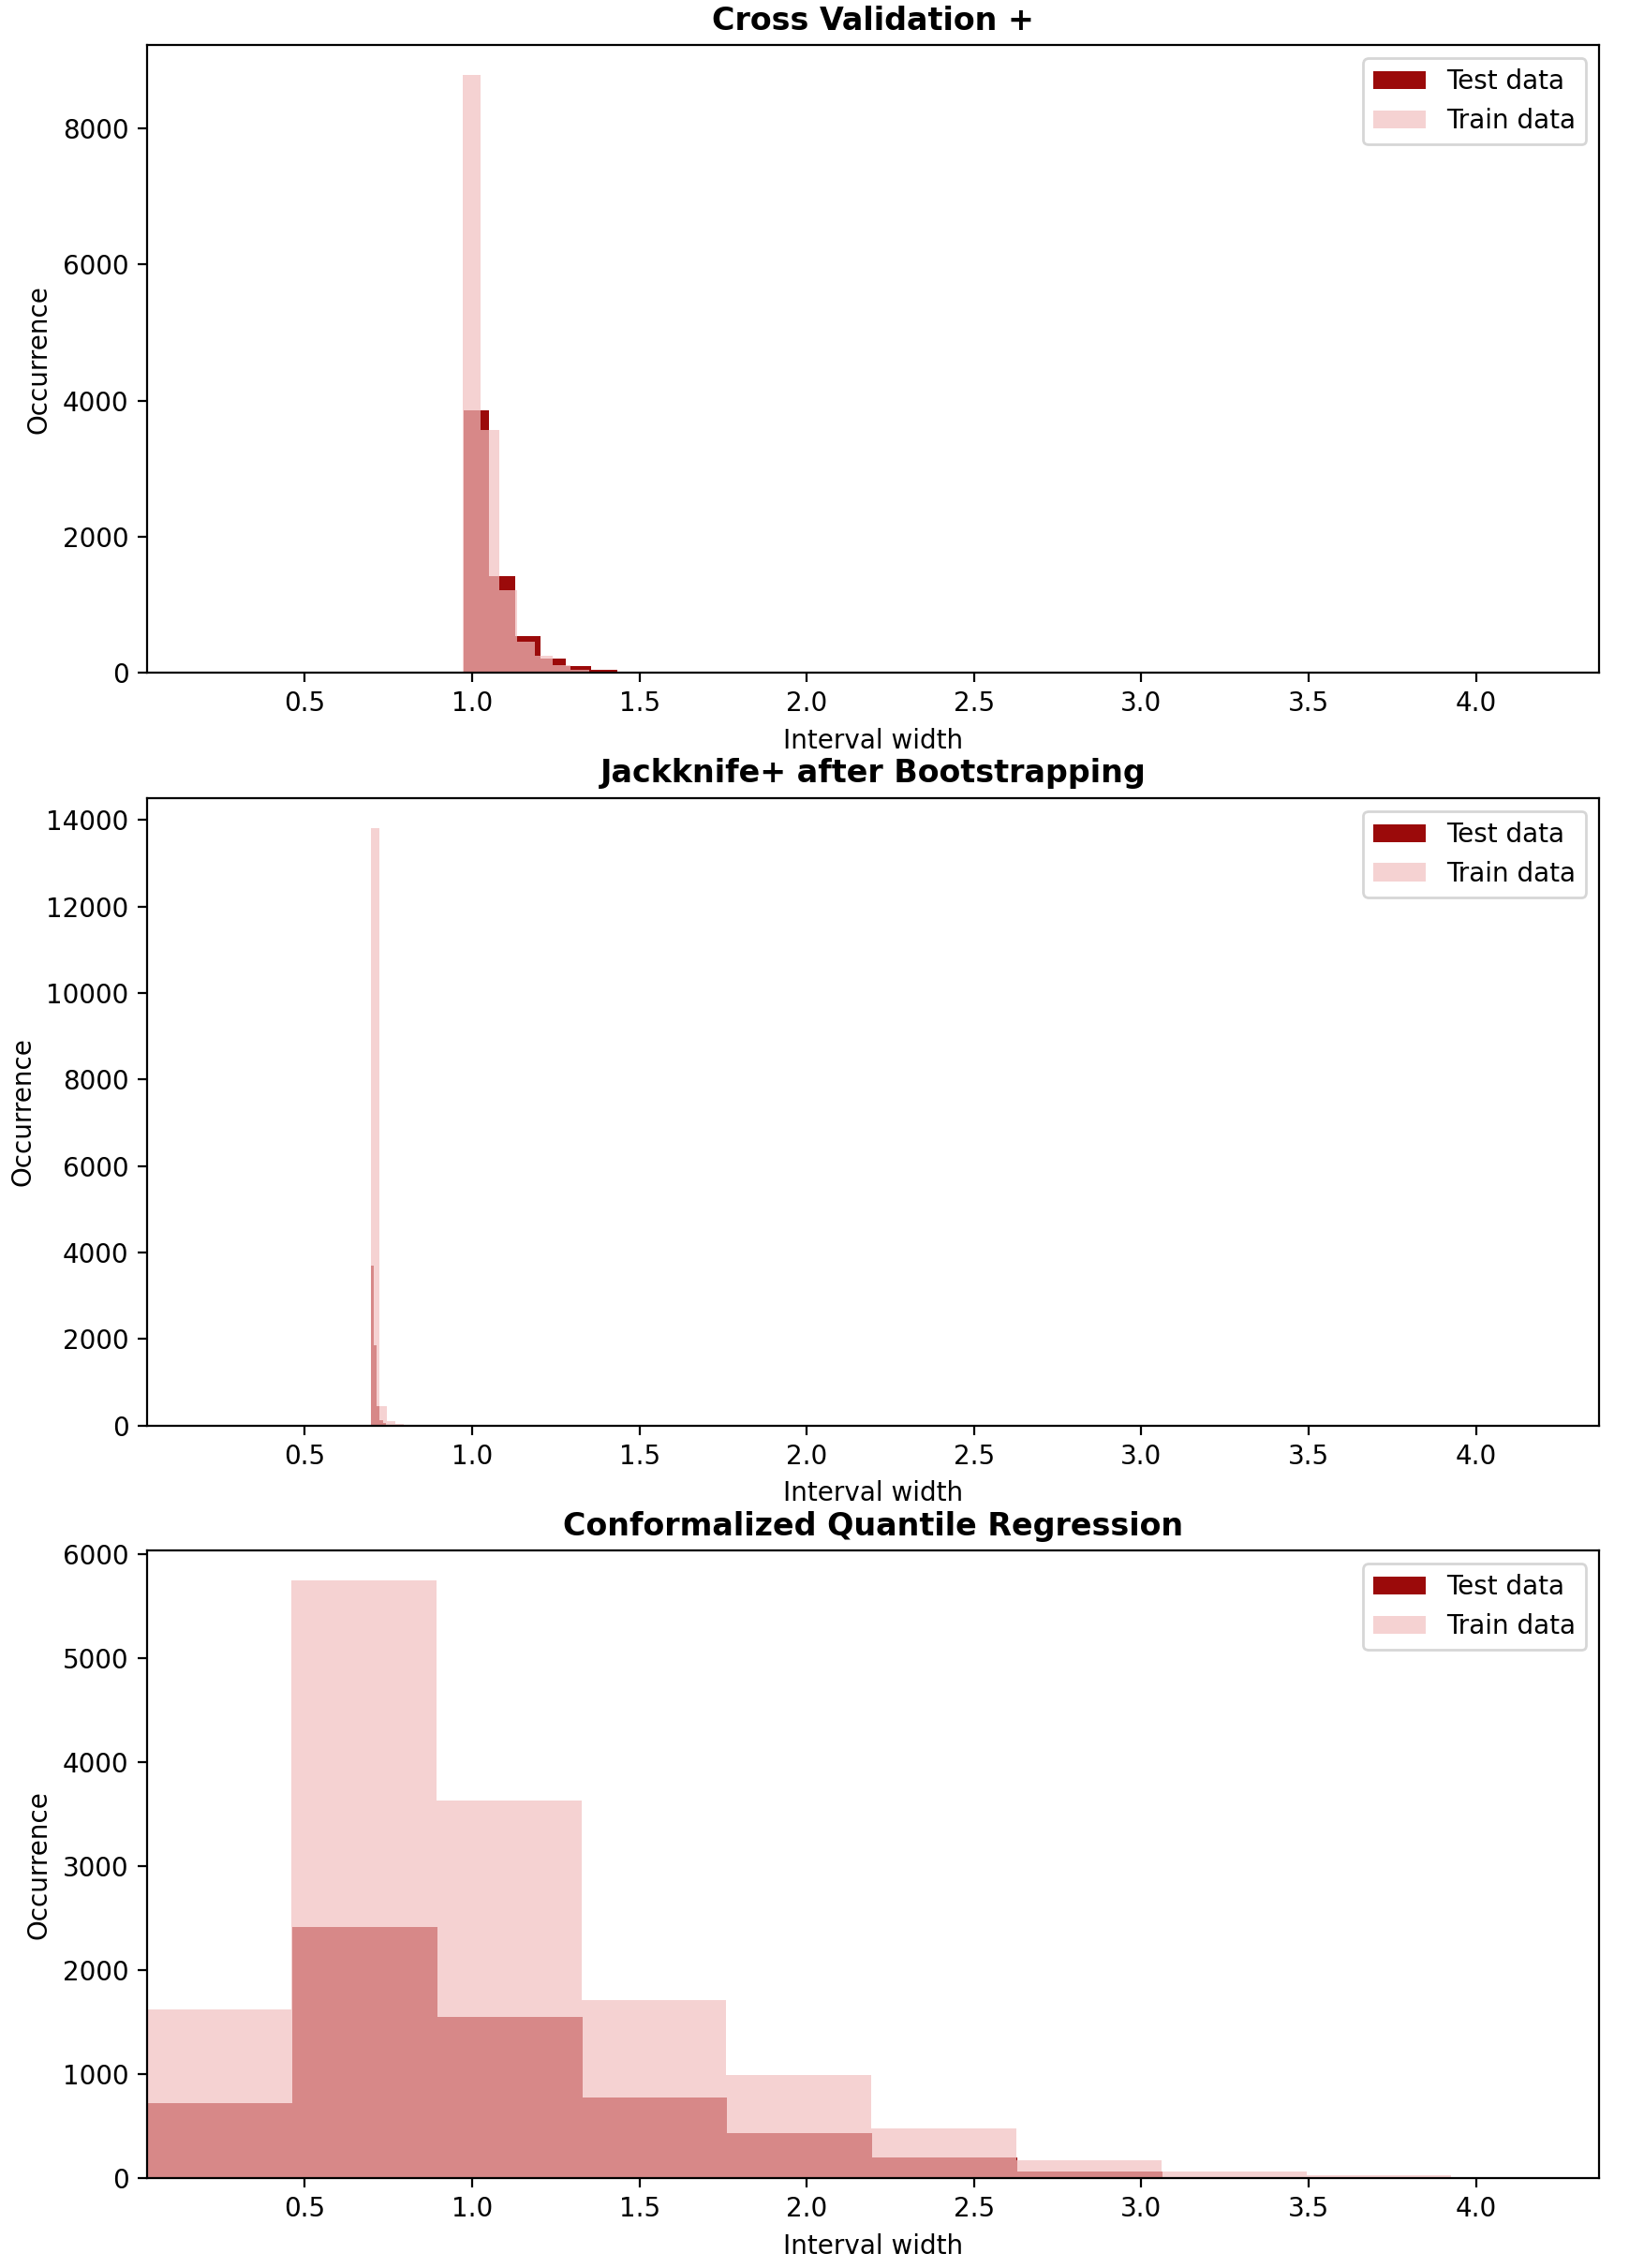
\includegraphics[width=\textwidth, height=1.9\textwidth]{Figures/regression/width-occurrence-regression-problem.png}
            % \caption{Intervals' width histograms}
        \end{subfigure}
        \hfill
        \begin{subfigure}[b]{0.32\textwidth}
            \centering
            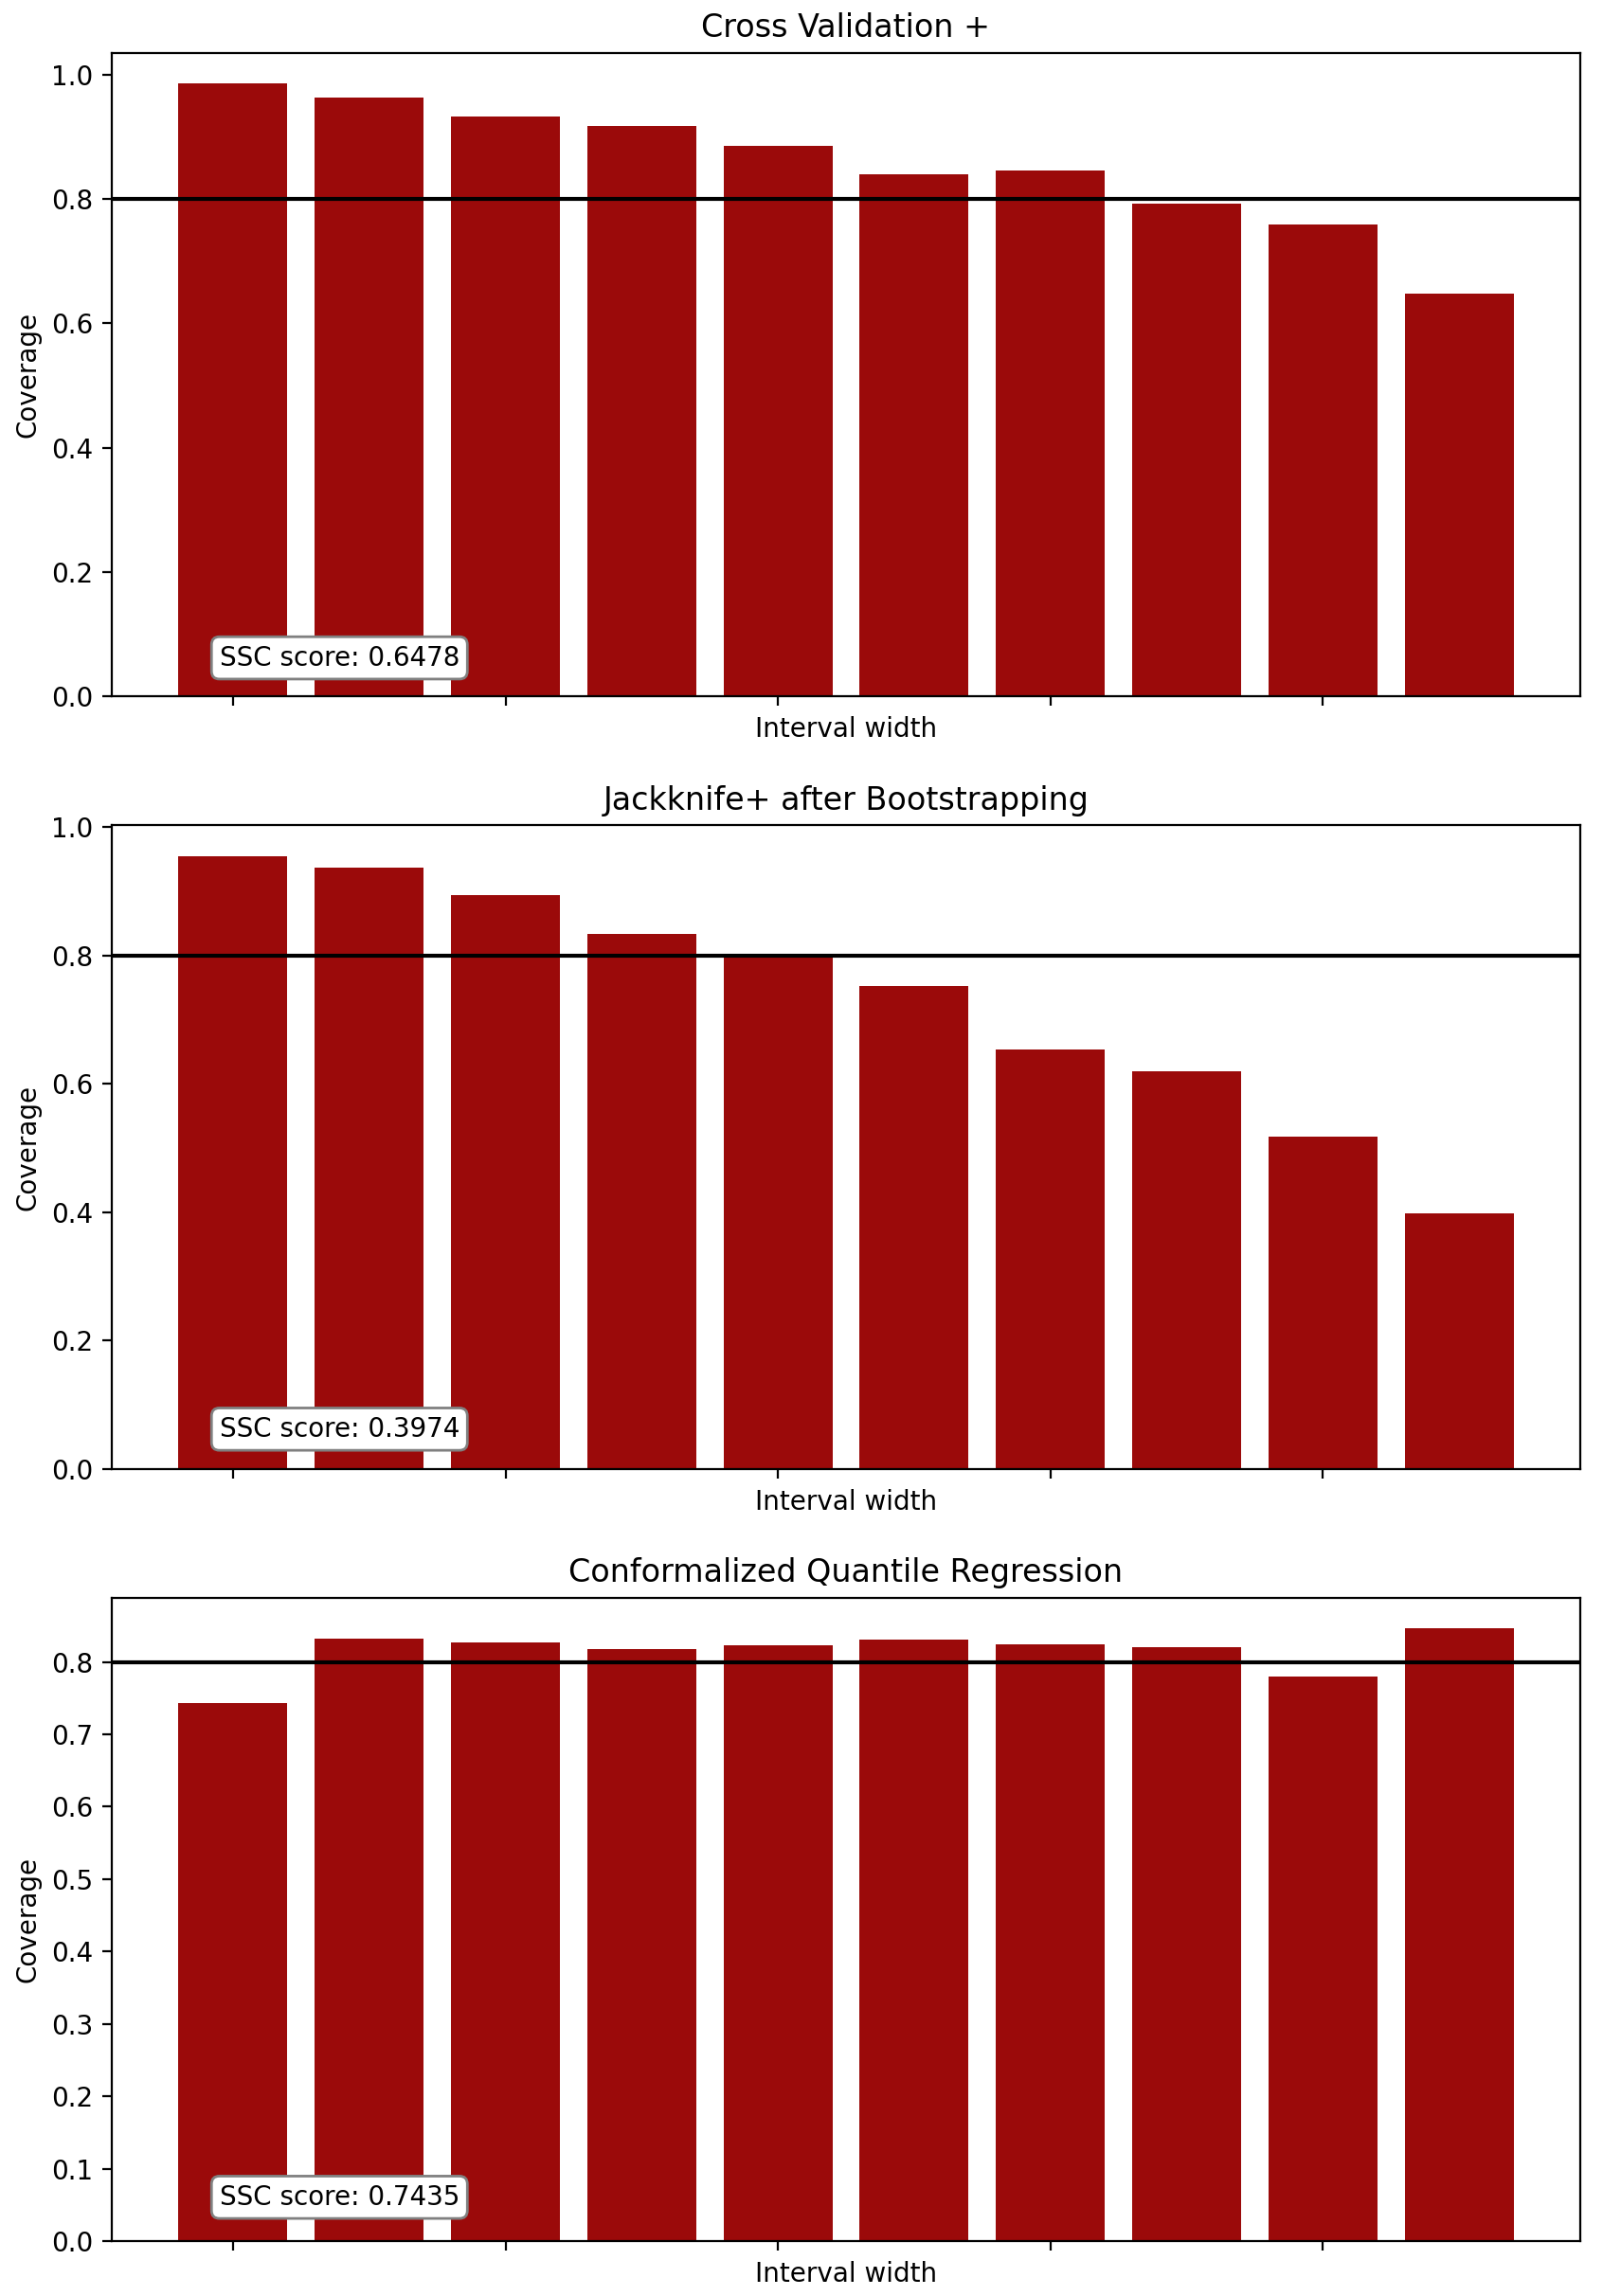
\includegraphics[width=\textwidth, height=1.9\textwidth]{Figures/regression/coverage-vs-width-regression-problem.png}
            % \caption{Coverage in function of intervals' width}
        \end{subfigure}
        \hfill % adds horizontal space between figures
        \begin{subfigure}[b]{0.32\textwidth} % Adjust the width to fit your needs
            \centering
            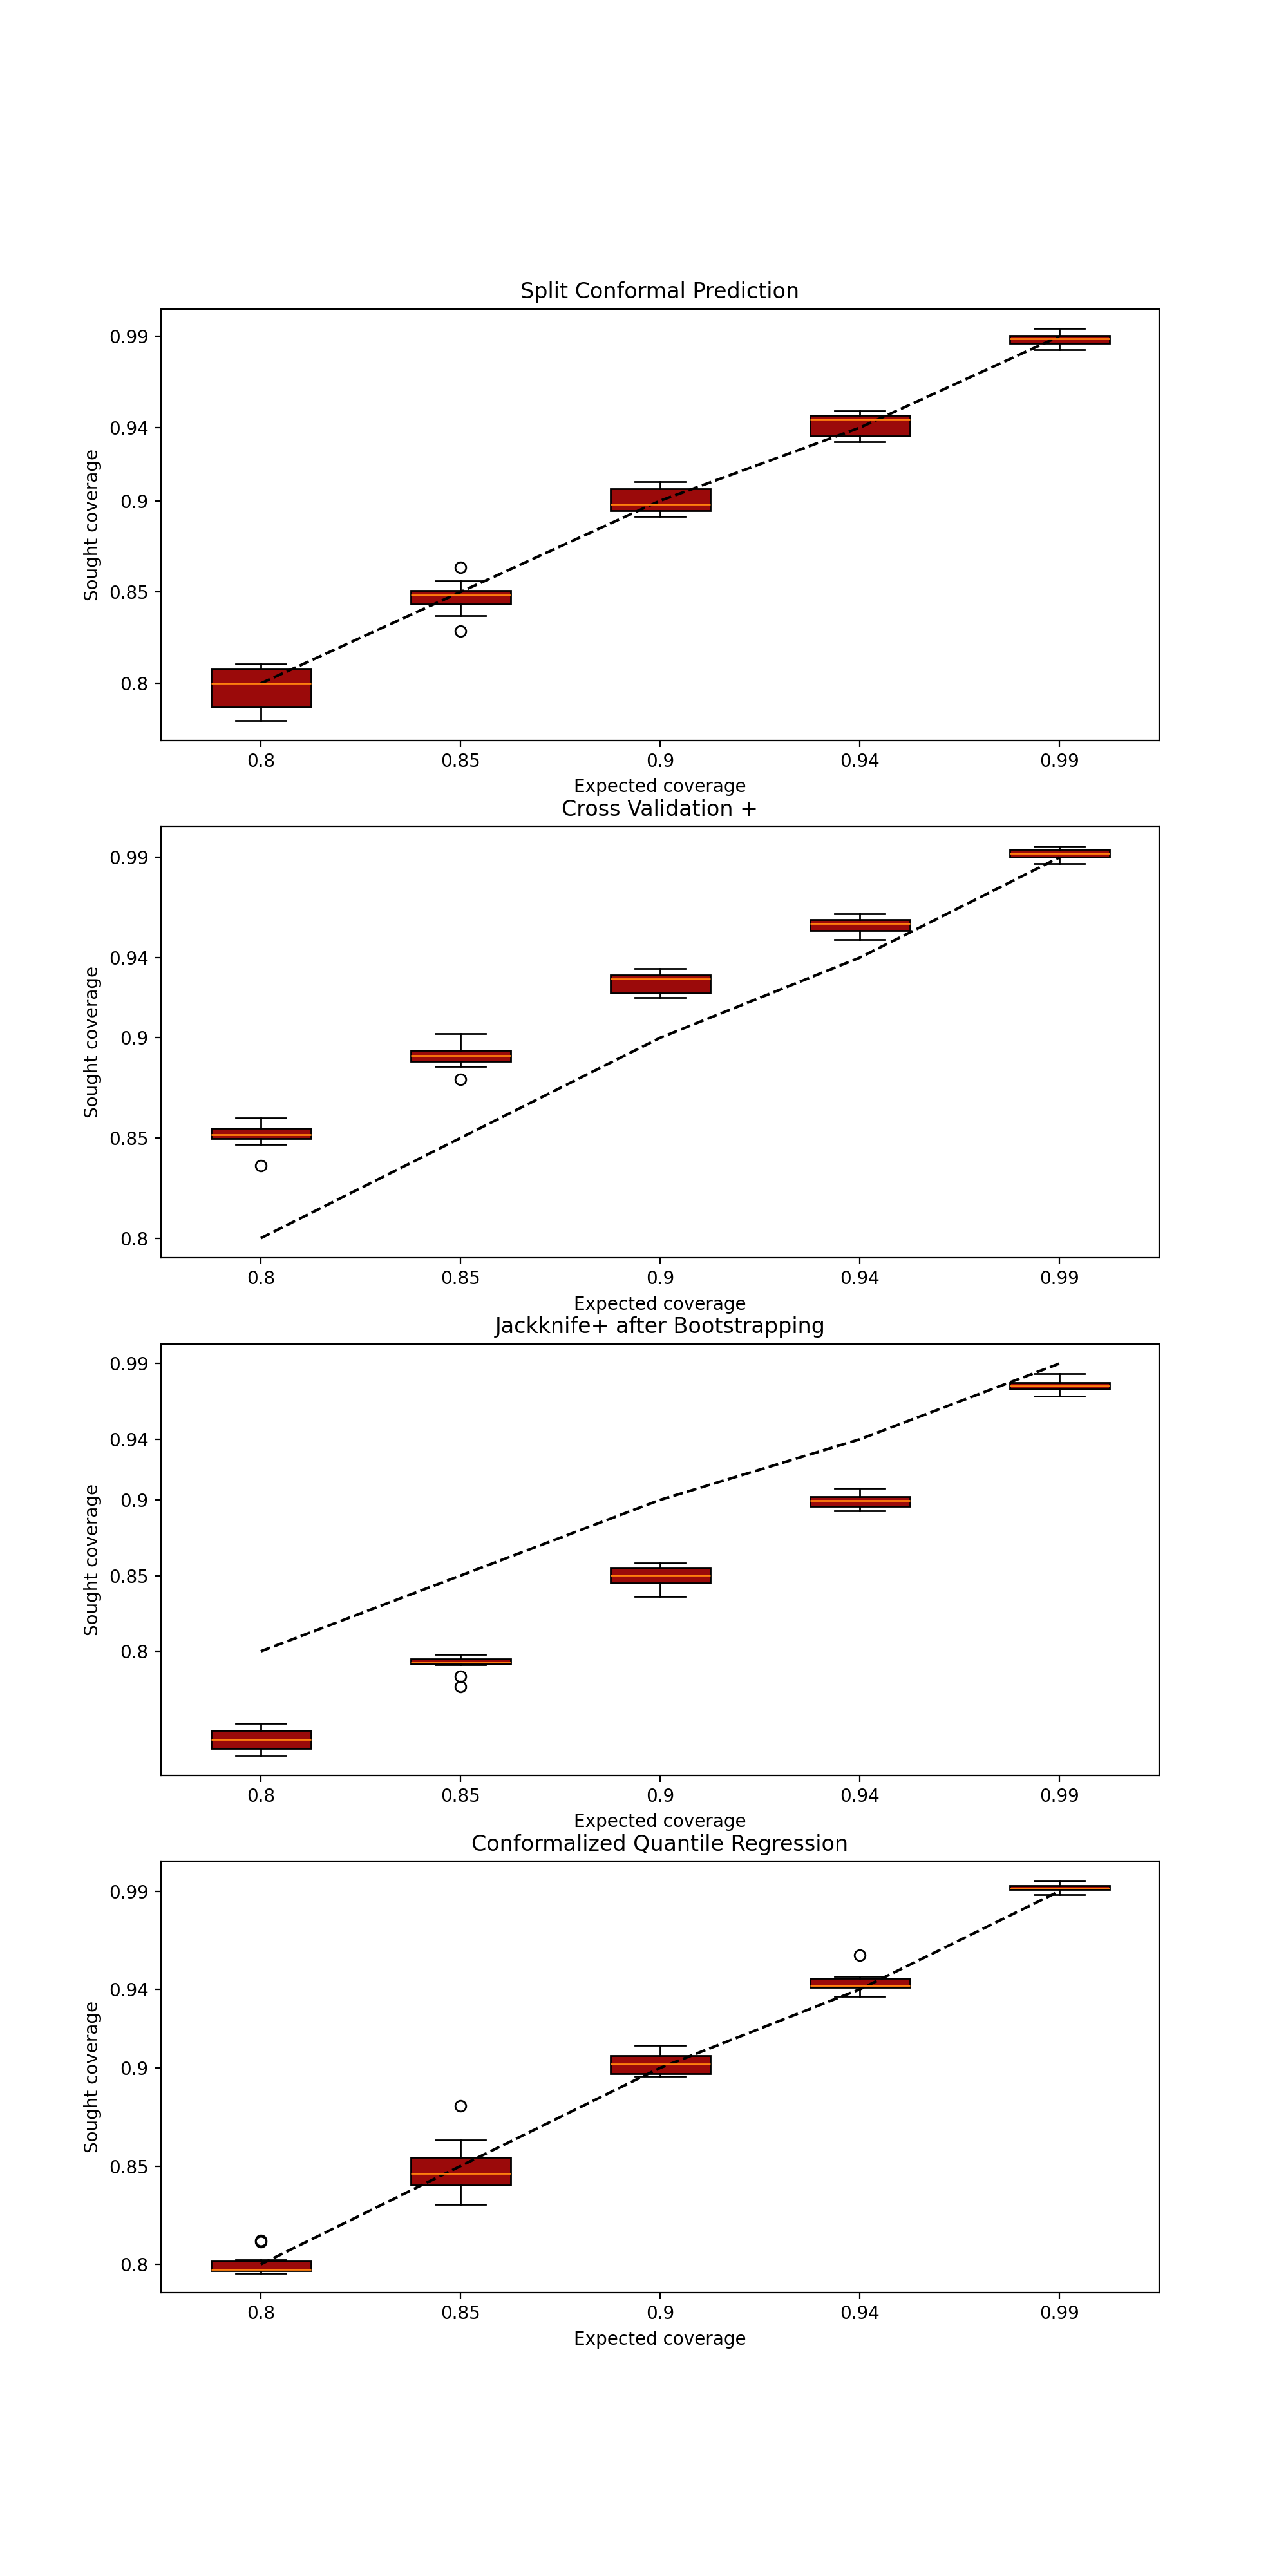
\includegraphics[width=\textwidth, height=1.9\textwidth]{Figures/regression/coverage-vs-alpha-regression-problem.png} % Adjust the filename and path
            % \caption{Coverage in function of $\a$}
        \end{subfigure}
        \caption{Width histograms \& coverage vs. width \& $\a$.}
        % \caption{Visualizations related to width \& coverage distributions for the test data and 4 different strategies, from top to bottom: SCP, CV$+$, J$+$aB \& CQR. The first 2 plots just display the last 3 strategies, since SCP displays no adaptability at all (whereas J$+$aB slight to none adaptability).}
    \end{figure}
\end{frame}

%% Time series problem %% (5pp)

\subsection{Time series problem}

%! Original dataset !% (2pp)

\subsubsection{Original dataset}

% Dataset %

\begin{frame}{Dataset}
        A time series forecasting problem is considered with:
        \begin{itemize}%[<+->][<+->]
            \item Victoria electricity demand dataset (1340 samples, features: time, demand lagged up to 7 days \& temperature).
            \item A \texttt{sklearn} random forest regressor automatically fine-tuned through grid-search.
            \item A 5-fold cross-validation for $\a=0.20$: % Figure \ref{fig:ts-splits}.
            \item[]<2->
            % \vspace{-2mm}
            \begin{figure}
                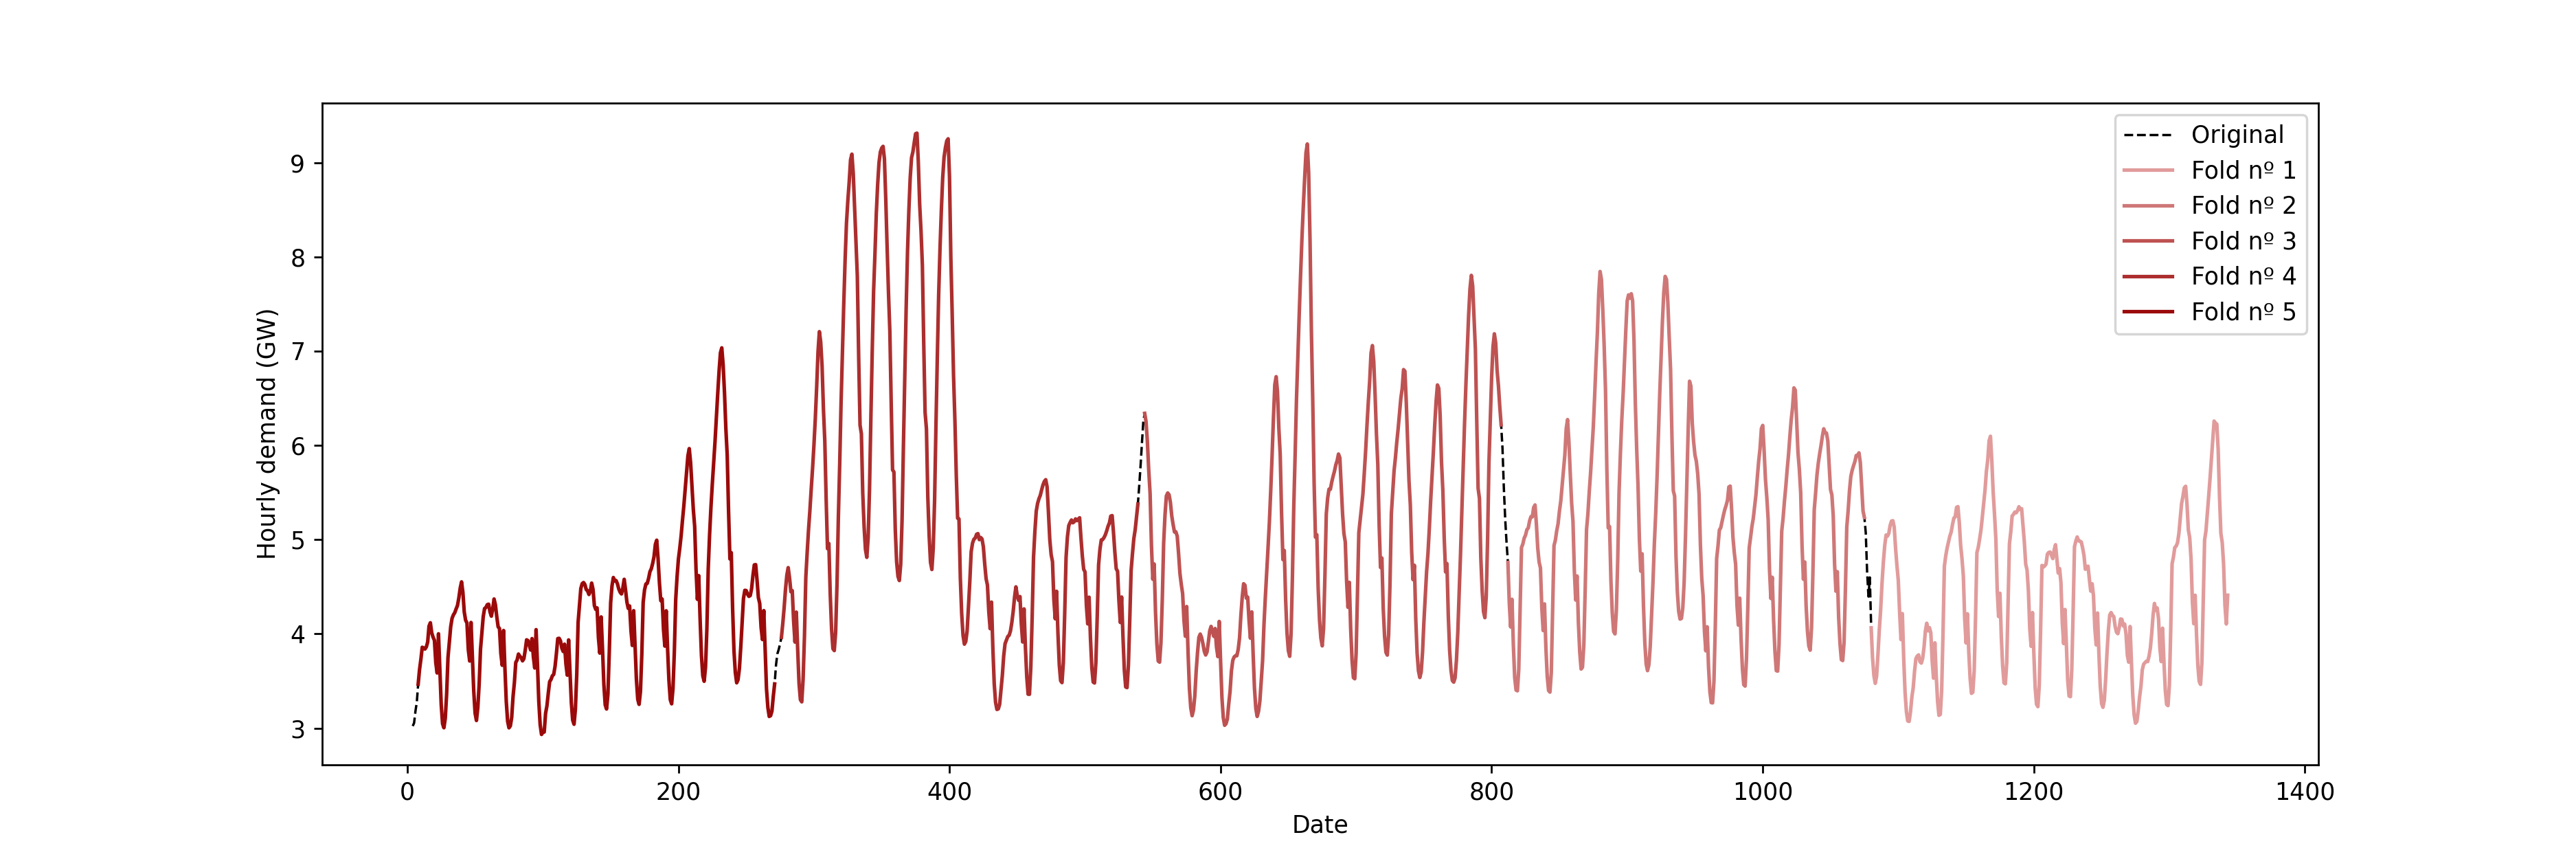
\includegraphics[width=0.9\textwidth]{Figures/timeseries/without-change-point/ts-5-folds.png}
                %\label{fig:ts-splits}
                \vspace{-2mm}
                \caption{5-fold CV splits.}
            \end{figure}
        \end{itemize}
\end{frame}

% Metrics table %

\begin{frame}{Metrics table}

    \begin{table}[ht]
        %\hspace{-5mm}
        \begin{subtable}{.5\textwidth}
            \hspace{-20mm}
            \begin{tabular}{|c|c|c|c|}
            \rowcolor{ColHead}\textcolor{white}{Strategy} & \textcolor{white}{Coverage} & \textcolor{white}{RMSE} & \textcolor{white}{Total time} \\ \hline
            \cellcolor{RowHead}{\small EnbPI\_{}nP} & 0.780 $\pm$ 0.069 & 0.165 $\pm$ 0.067 & 6.2 $\pm$ 0.3 \\
            \cellcolor{RowHead}{\small EnbPI} & 0.789 $\pm$ 0.058 & 0.165 $\pm$ 0.067 & 528.3 $\pm$ 0.4\\
            \hline
            \end{tabular}
        % \caption{Coverage, RMSE, total time (training \& inference with residuals adjustment if applies).}
        \label{subtab:timeseries-metrics-1}
        \end{subtable}
        
        \begin{subtable}{.5\textwidth}
            \hspace{-35mm}
            \begin{tabular}{|c|c|c|c|c|}
            \rowcolor{ColHead}\textcolor{white}{Strategy} & \textcolor{white}{Coverage} & \textcolor{white}{Width} & \textcolor{white}{CWC} & \textcolor{white}{SSC} \\ \hline
            \cellcolor{RowHead}{\small EnbPI\_{}nP} & 0.780 $\pm$ 0.069 & 0.293 $\pm$ 0.013 & 0.935 $\pm$ 0.018 & ---  \\
            \cellcolor{RowHead}{\small EnbPI} & 0.789 $\pm$ 0.058 & 0.300 $\pm$ 0.007 & 0.93 $\pm$ 0.02 & 0.5 $\pm$ 0.2\\
            \hline
            \end{tabular}
        % \caption{Coverage, width, coverage width-based criterion (CWC) score \& size-stratified coverage (SSC) score}
        % \label{subtab:timeseries-metrics-2}
        \end{subtable}
        
    \end{table}
\end{frame}

% Other visualizations %

\begin{frame}{Other visualizations}
    \vspace{-5mm}
    \begin{figure}[ht]
        \centering
        %\hspace{-10mm}
        \begin{subfigure}[b]{0.32\textwidth}
            \centering
            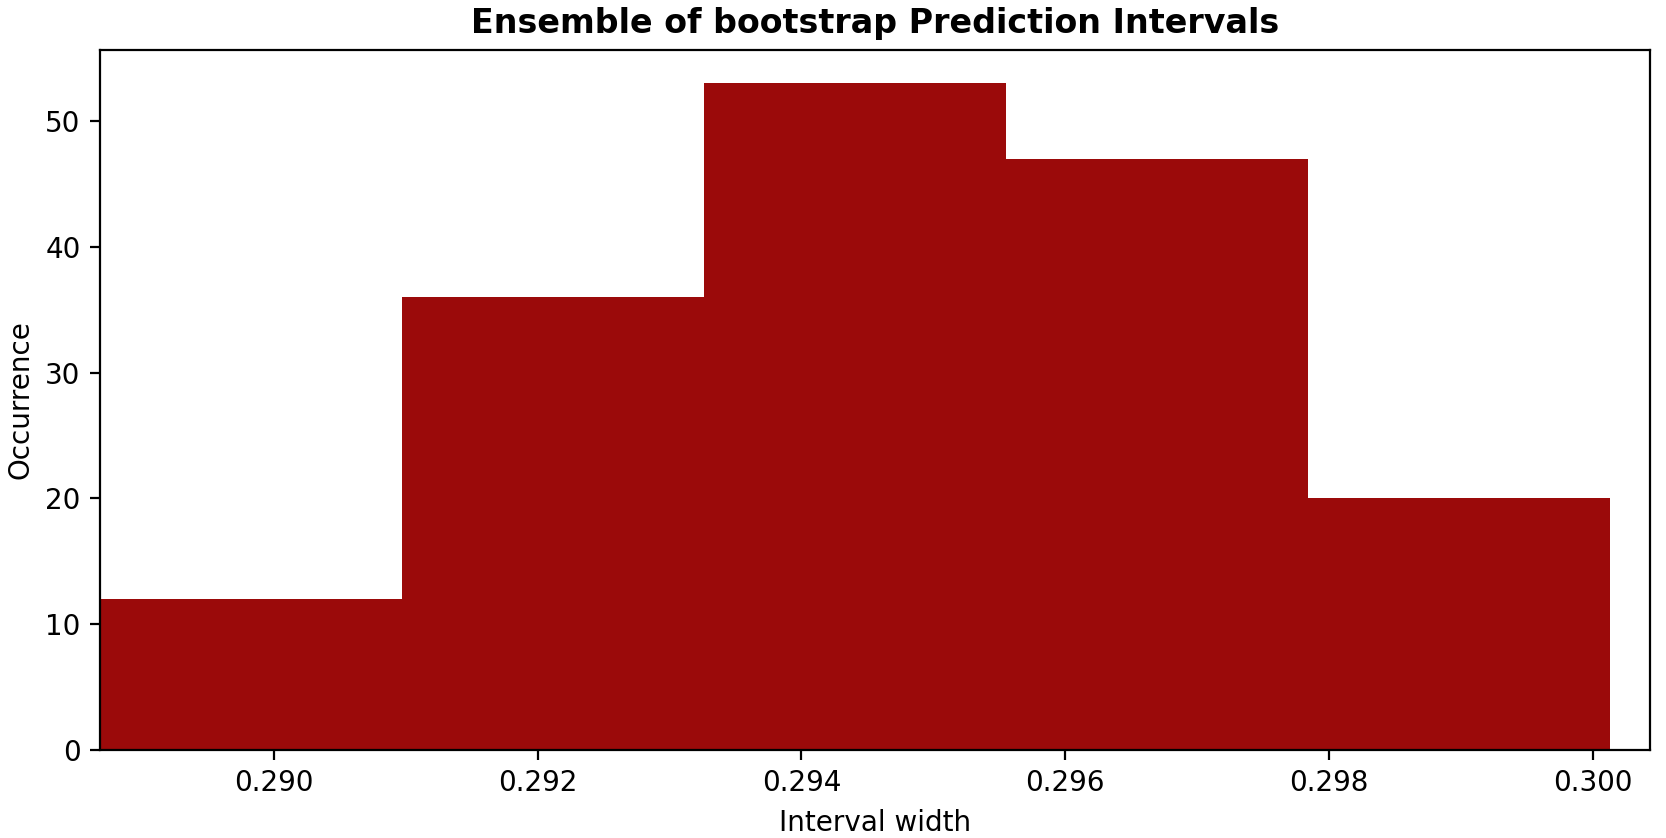
\includegraphics[width=1.05\textwidth, height=1.1\textwidth]{Figures/timeseries/without-change-point/width-occurrence-timeseries-problem.png}
            \caption{EnbPI intervals' width histograms}
        \end{subfigure}
        \hfill
        \begin{subfigure}[b]{0.32\textwidth}
            \centering
            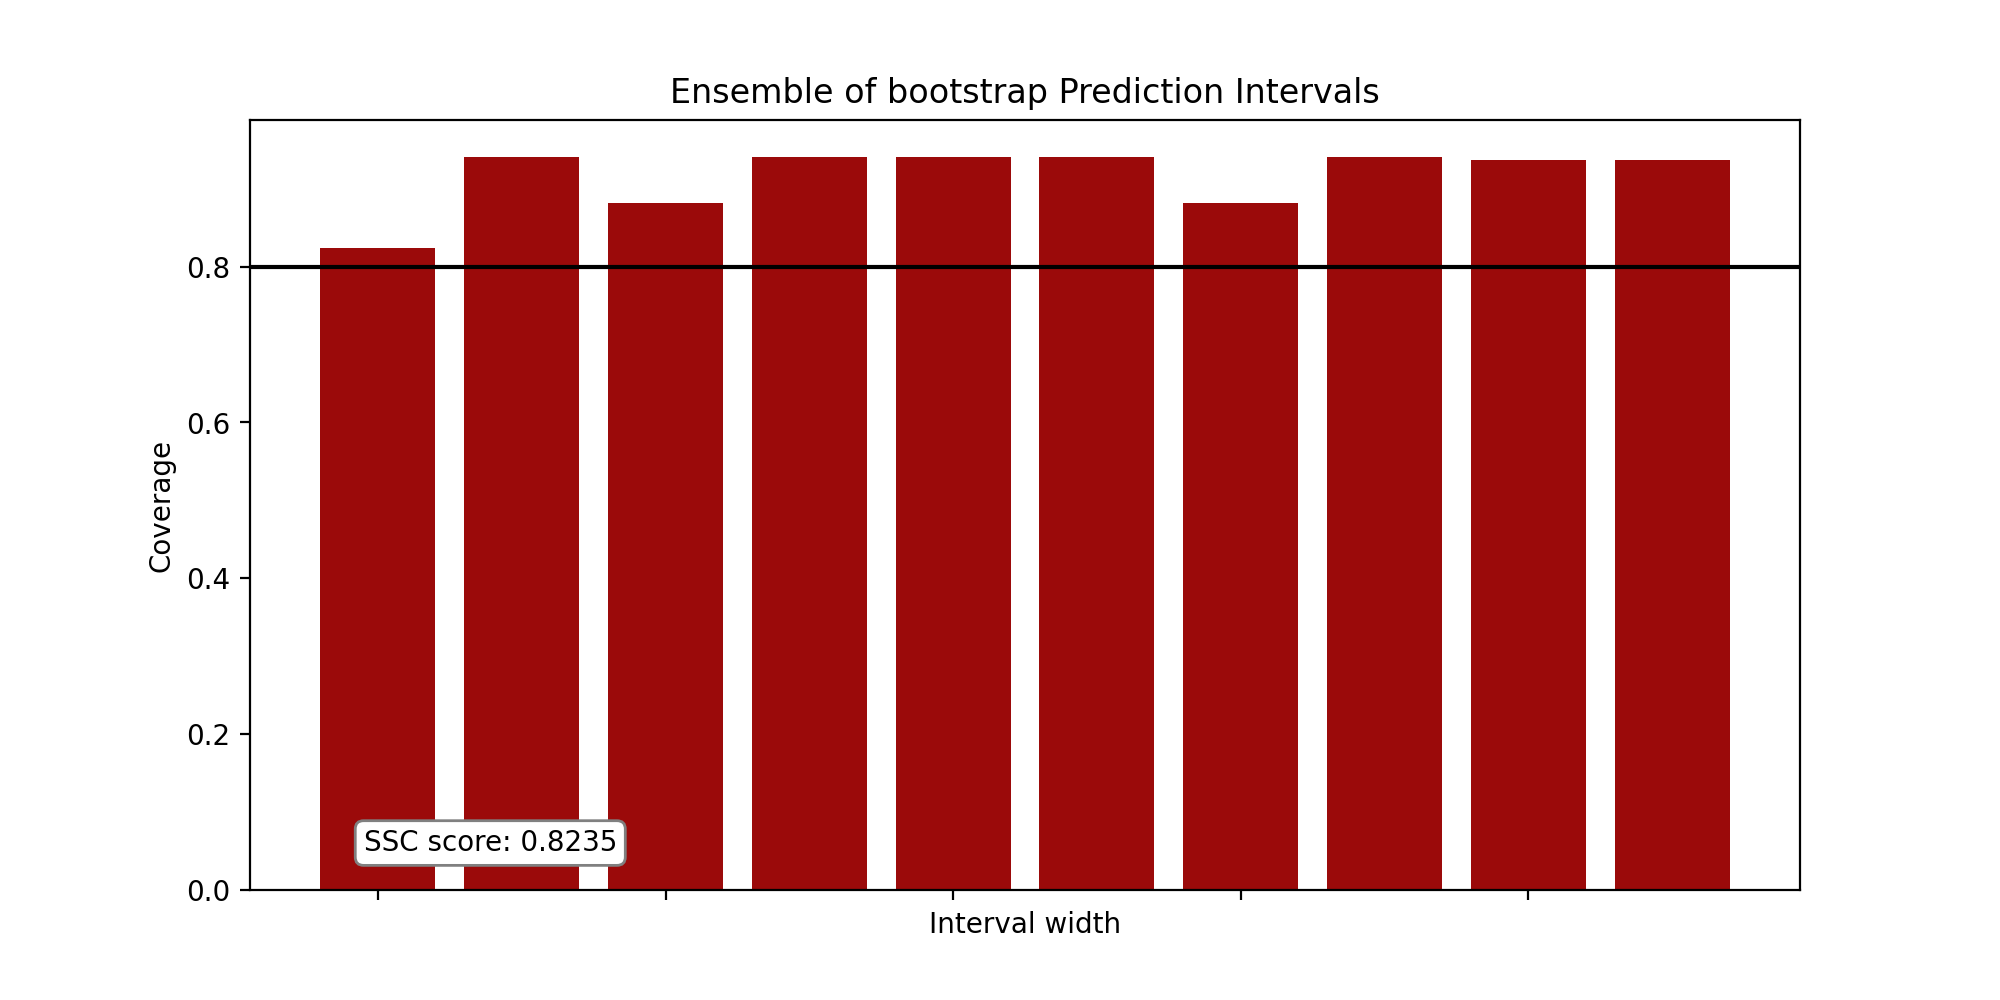
\includegraphics[width=1.05\textwidth, height=1.1\textwidth]{Figures/timeseries/without-change-point/coverage-vs-width-timeseries-problem.png}
            \caption{EnbPI coverage in function of intervals' width}
        \end{subfigure}
        \hfill % adds horizontal space between figures
        \begin{subfigure}[b]{0.32\textwidth} % Adjust the width to fit your needs
            \centering
            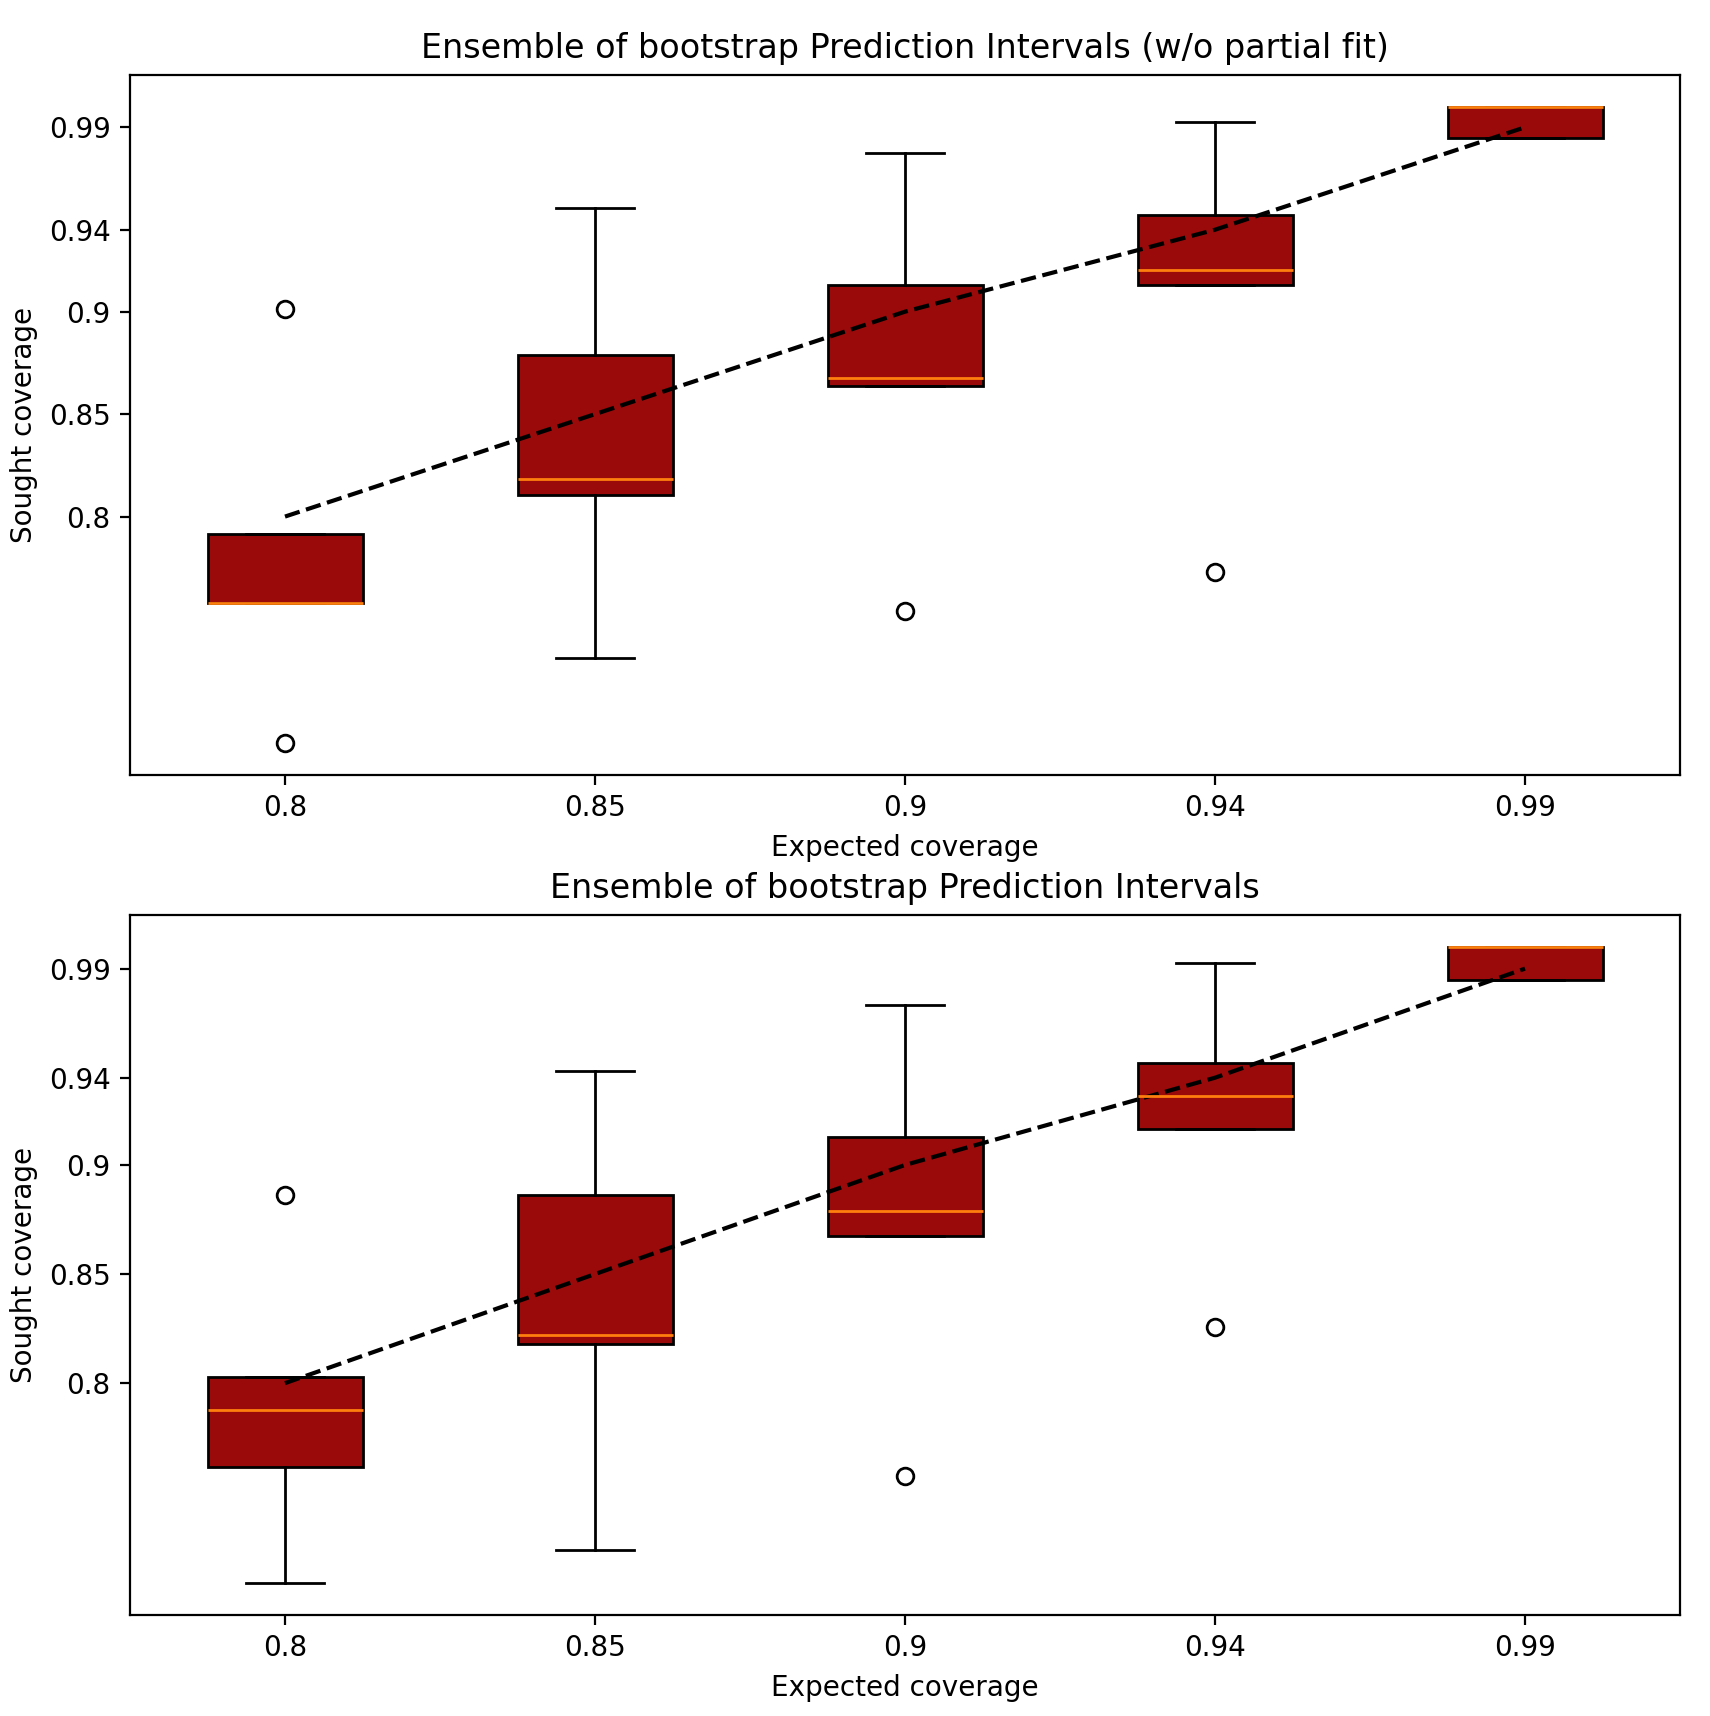
\includegraphics[width=1.05\textwidth, height=1.3\textwidth]{Figures/timeseries/without-change-point/coverage-vs-alpha-timeseries-problem.png} % Adjust the filename and path
            \caption{EnbPI\_{}nP \& EnbPI coverage in function of $\a$}
        \end{subfigure}
        \caption{Width histograms \& coverage vs. width \& $\a$.}
        % \caption{Visualizations related to width \& coverage distributions for the test data and 4 different strategies, from top to bottom: SCP, CV$+$, J$+$aB \& CQR. The first 2 plots just display the last 3 strategies, since SCP displays no adaptability at all (whereas J$+$aB slight to none adaptability).}
    \end{figure}
\end{frame}

%! Change point in test !% (3pp)

\subsubsection{Change point in test}

% Dataset %

\begin{frame}{Idea}
    The consistency of former time series may outshine the benefits of the "\textit{partial fit}" EnbPI feature. Thus:
    \begin{itemize}%[<+->][<+->]
        \item A change point is added in test to mock off a distribution shift.
        \item The same random forest regressor will be applied to a 5-fold cross-validation, now for $\a=0.05$: % Figure \ref{fig:ts-splits-cpoint}.
        \item[]
            \hspace{-5mm}
            \vspace{-7mm}
            \begin{figure}
                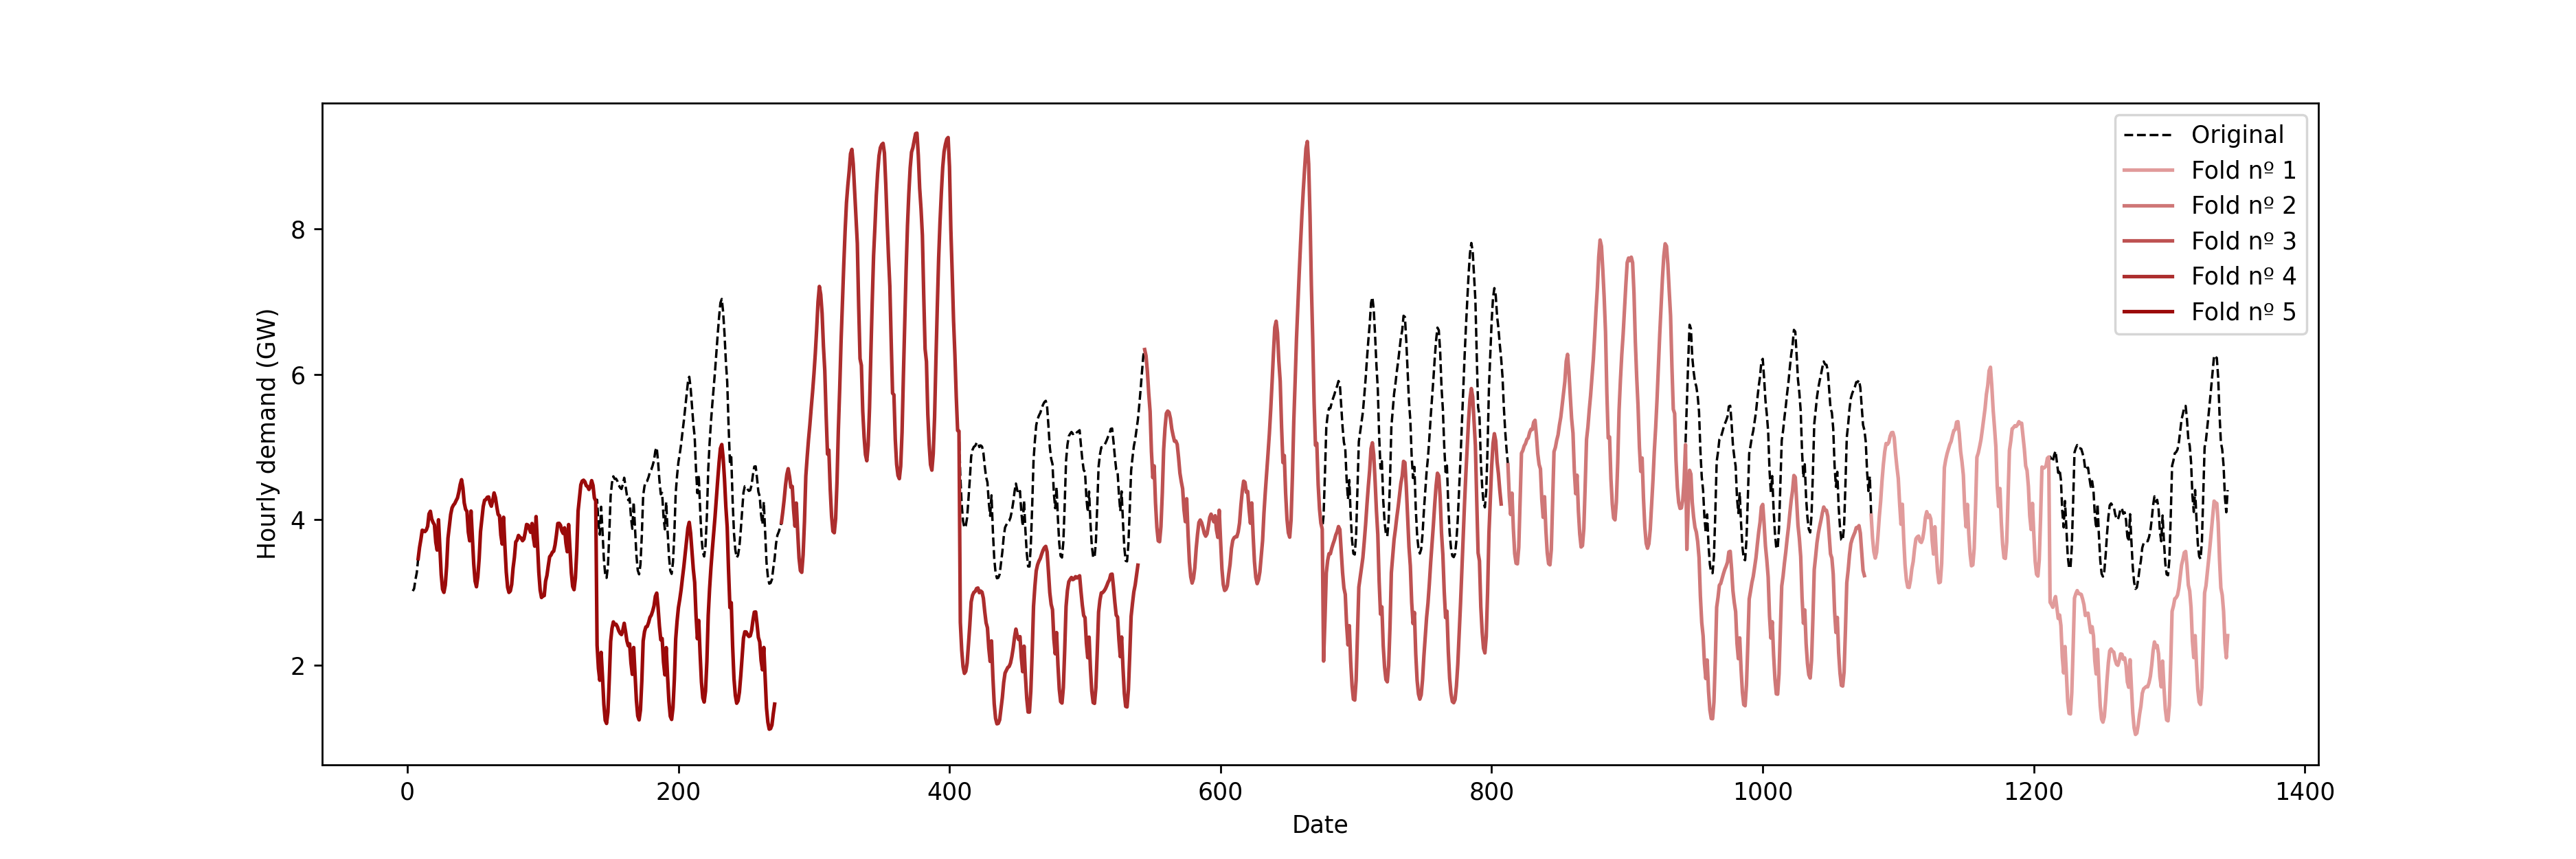
\includegraphics[width=\textwidth]{Figures/timeseries/with-change-point/ts-with-change-point-5-folds.png}
                \label{fig:ts-splits-cpoint}
                \vspace{-2mm}
                \caption{5-fold CV splits with change points in each test's.}
        \end{figure} 
    \end{itemize}
\end{frame}

% Metrics & plots %

\begin{frame}{Metrics \& plot}

\begin{minipage}{\textwidth}
\begin{table}[ht]
    \hspace{-5mm}
    \begin{subtable}{.5\textwidth}
        \hspace{-16mm}
        \begin{tabular}{|c|c|c|c|}
            \rowcolor{ColHead}\textcolor{white}{Strategy} & \textcolor{white}{Coverage} & \textcolor{white}{RMSE} & \textcolor{white}{Total time} \\ \hline
            \cellcolor{RowHead}{\small EnbPI\_{}nP} & 0.439 $\pm$ 0.075 & 1.431 $\pm$ 0.024 & 6.0 $\pm$ 0.3 \\
            \cellcolor{RowHead}{\small EnbPI} & 0.696 $\pm$ 0.042 & 1.431 $\pm$ 0.024 & 530 $\pm$ 1\\
            \hline
        \end{tabular}
        % \caption{Coverage, RMSE, total time (training \& inference with residuals adjustment if applies).}
        % \label{subtab:timeseries-metrics-1-cpoint}
    \end{subtable}

    \begin{subtable}{.5\textwidth}
        \hspace{-20mm}
        \begin{tabular}{|c|c|c|c|}
            \rowcolor{ColHead}\textcolor{white}{Strategy} & \textcolor{white}{Coverage} & \textcolor{white}{Width} %& \textcolor{white}{CWC} 
            & \textcolor{white}{SSC} \\ \hline
            \cellcolor{RowHead}{\small EnbPI\_{}nP} & 0.439 $\pm$ 0.075 & 0.569 $\pm$ 0.043 % & --- %0.899 $\pm$ 0.031 
            & --- \\
            \cellcolor{RowHead}{\small EnbPI} & 0.696 $\pm$ 0.042 & 1.300 $\pm$ 0.034 % & --- %0.777 $\pm$ 0.060 
            & 0.07 $\pm$ 0.12\\
            \hline
        \end{tabular}
        % \caption{Coverage, width, coverage width-based criterion (CWC) score \& size-stratified coverage (SSC) score}
        % \label{subtab:timeseries-metrics-2}
    \end{subtable}
\end{table}

\vspace{-5mm}
\end{minipage}
\vfill
% PLOTS

\begin{minipage}{\textwidth}

    \begin{columns} % the "c" option specifies center vertical alignment
        \vspace{-5mm}
        \begin{column}{0.5\textwidth}
            \centering
            %\hspace{-10mm}
            \begin{figure} %[b]{0.4\textwidth}
                \centering
                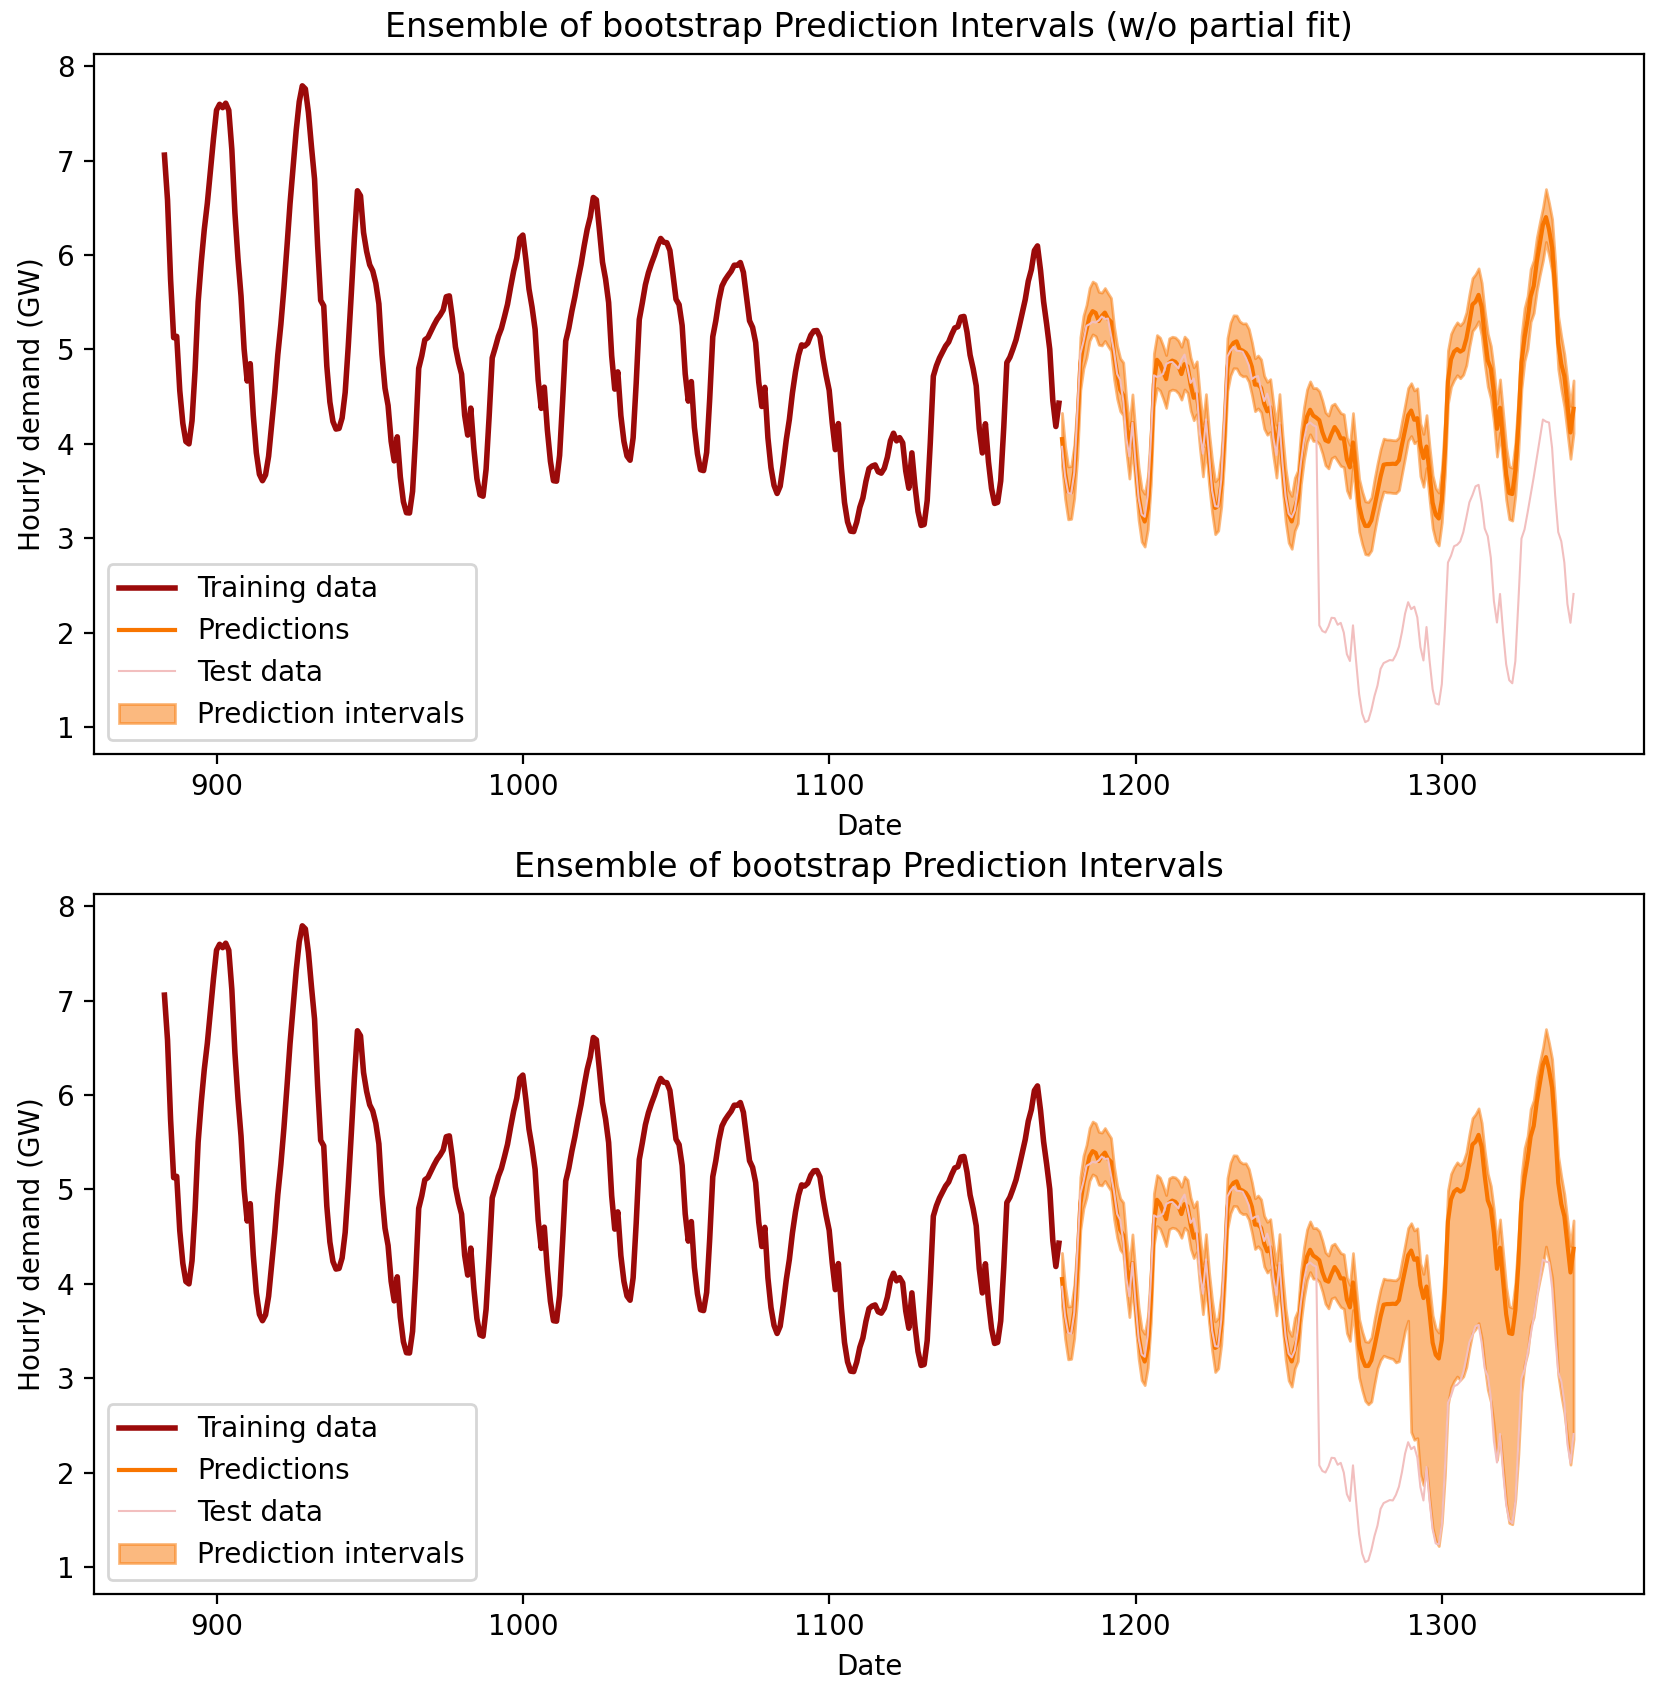
\includegraphics[width=0.8\textwidth, height=0.75\textwidth]{Figures/timeseries/with-change-point/prediction-intervals-timeseries-problem-with-change-point.png}
                % \caption{Coverage in function of time (grouped within 24h rolling windows) for the EnbPI strategies (and change point's data).}
            \end{figure}
        \end{column}
        \begin{column}{0.5\textwidth}
            \vspace{-7mm}
            \begin{figure}
                \centering
                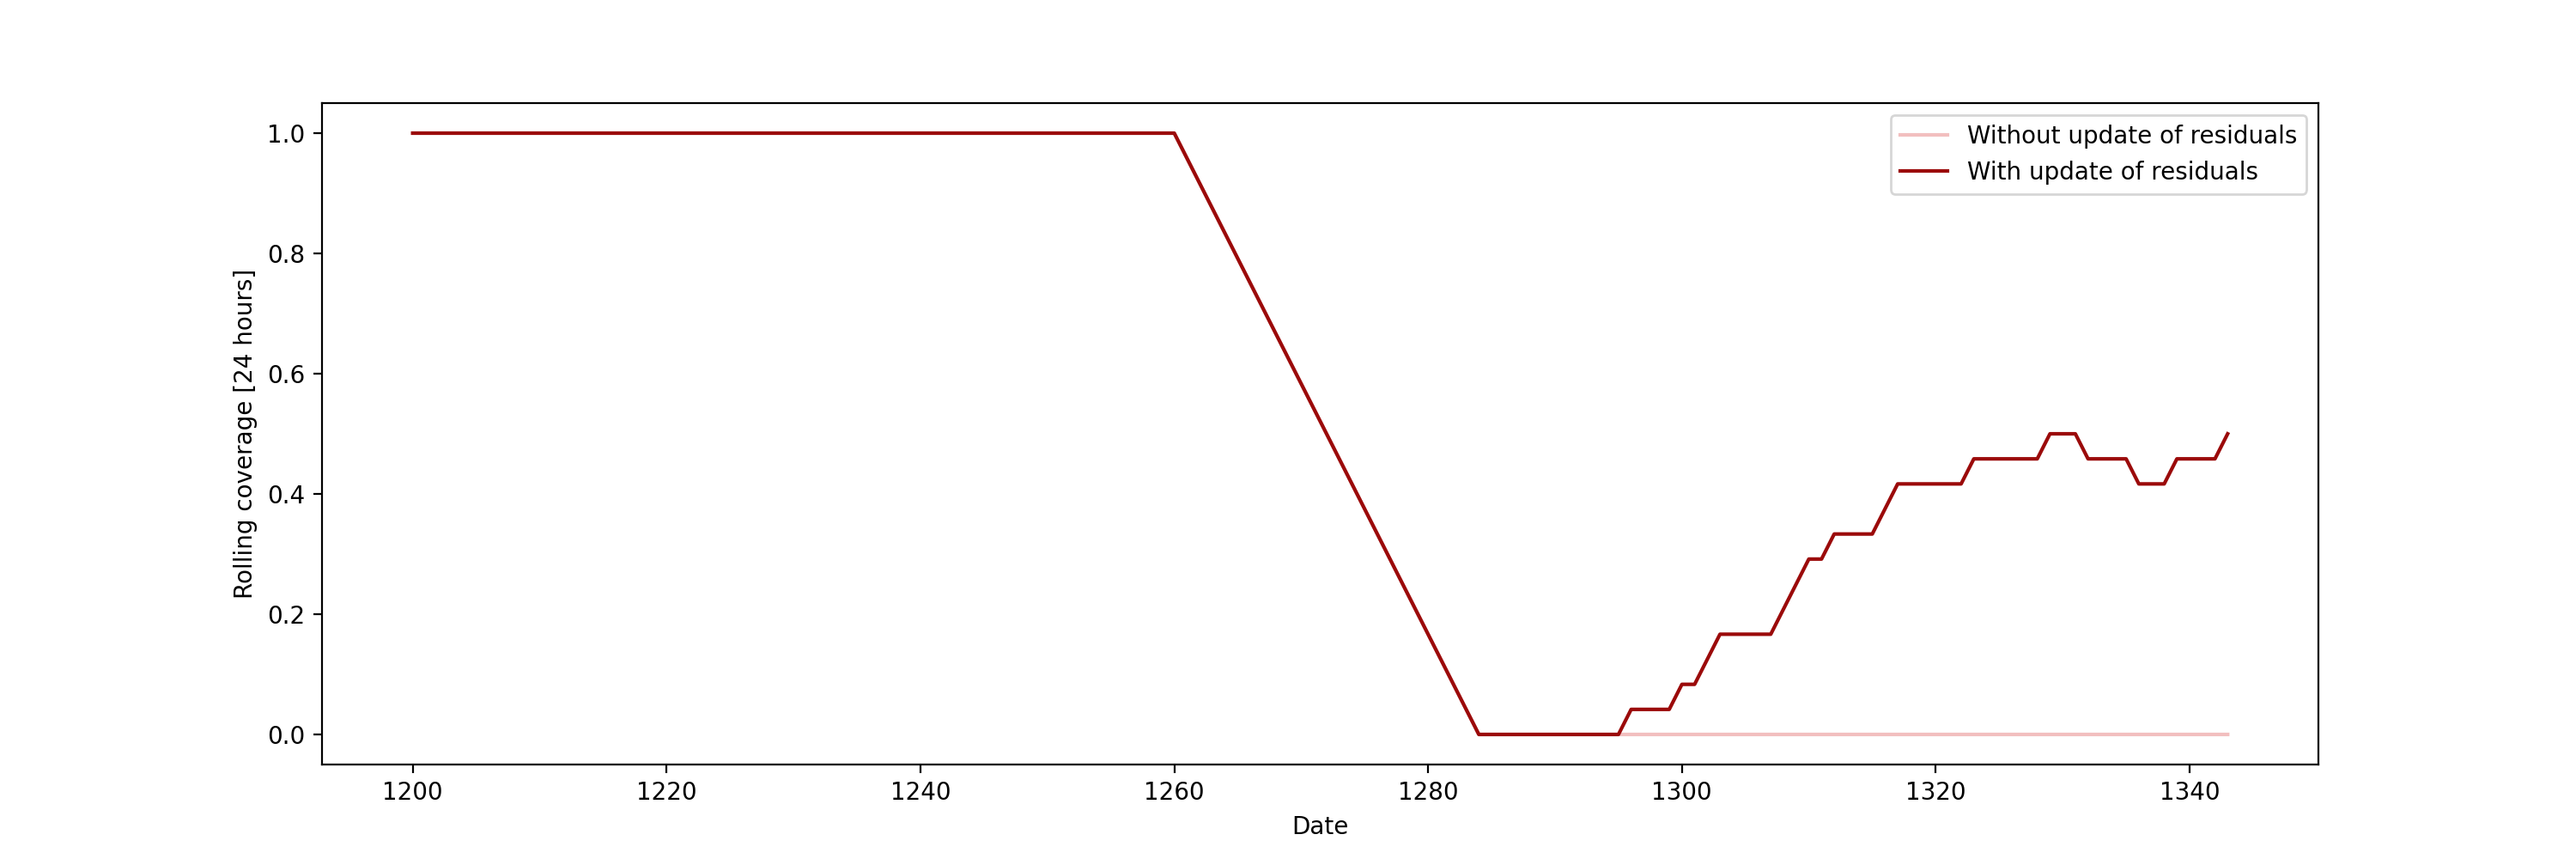
\includegraphics[width=\textwidth, height=0.5\textwidth]{Figures/timeseries/with-change-point/rolling-coverage-with-change-point.png}
                % \caption{Coverage in function of time (grouped within 24h rolling windows) for the EnbPI strategies (and change point's data).}
            \end{figure}
        \end{column}
    \end{columns}
\end{minipage}

% END OF FRAME 

\end{frame}

% Other visualizations %

% \begin{frame}{Other visualizations}
% \vspace{-2mm}
% \begin{figure}[ht]
%     \centering
%     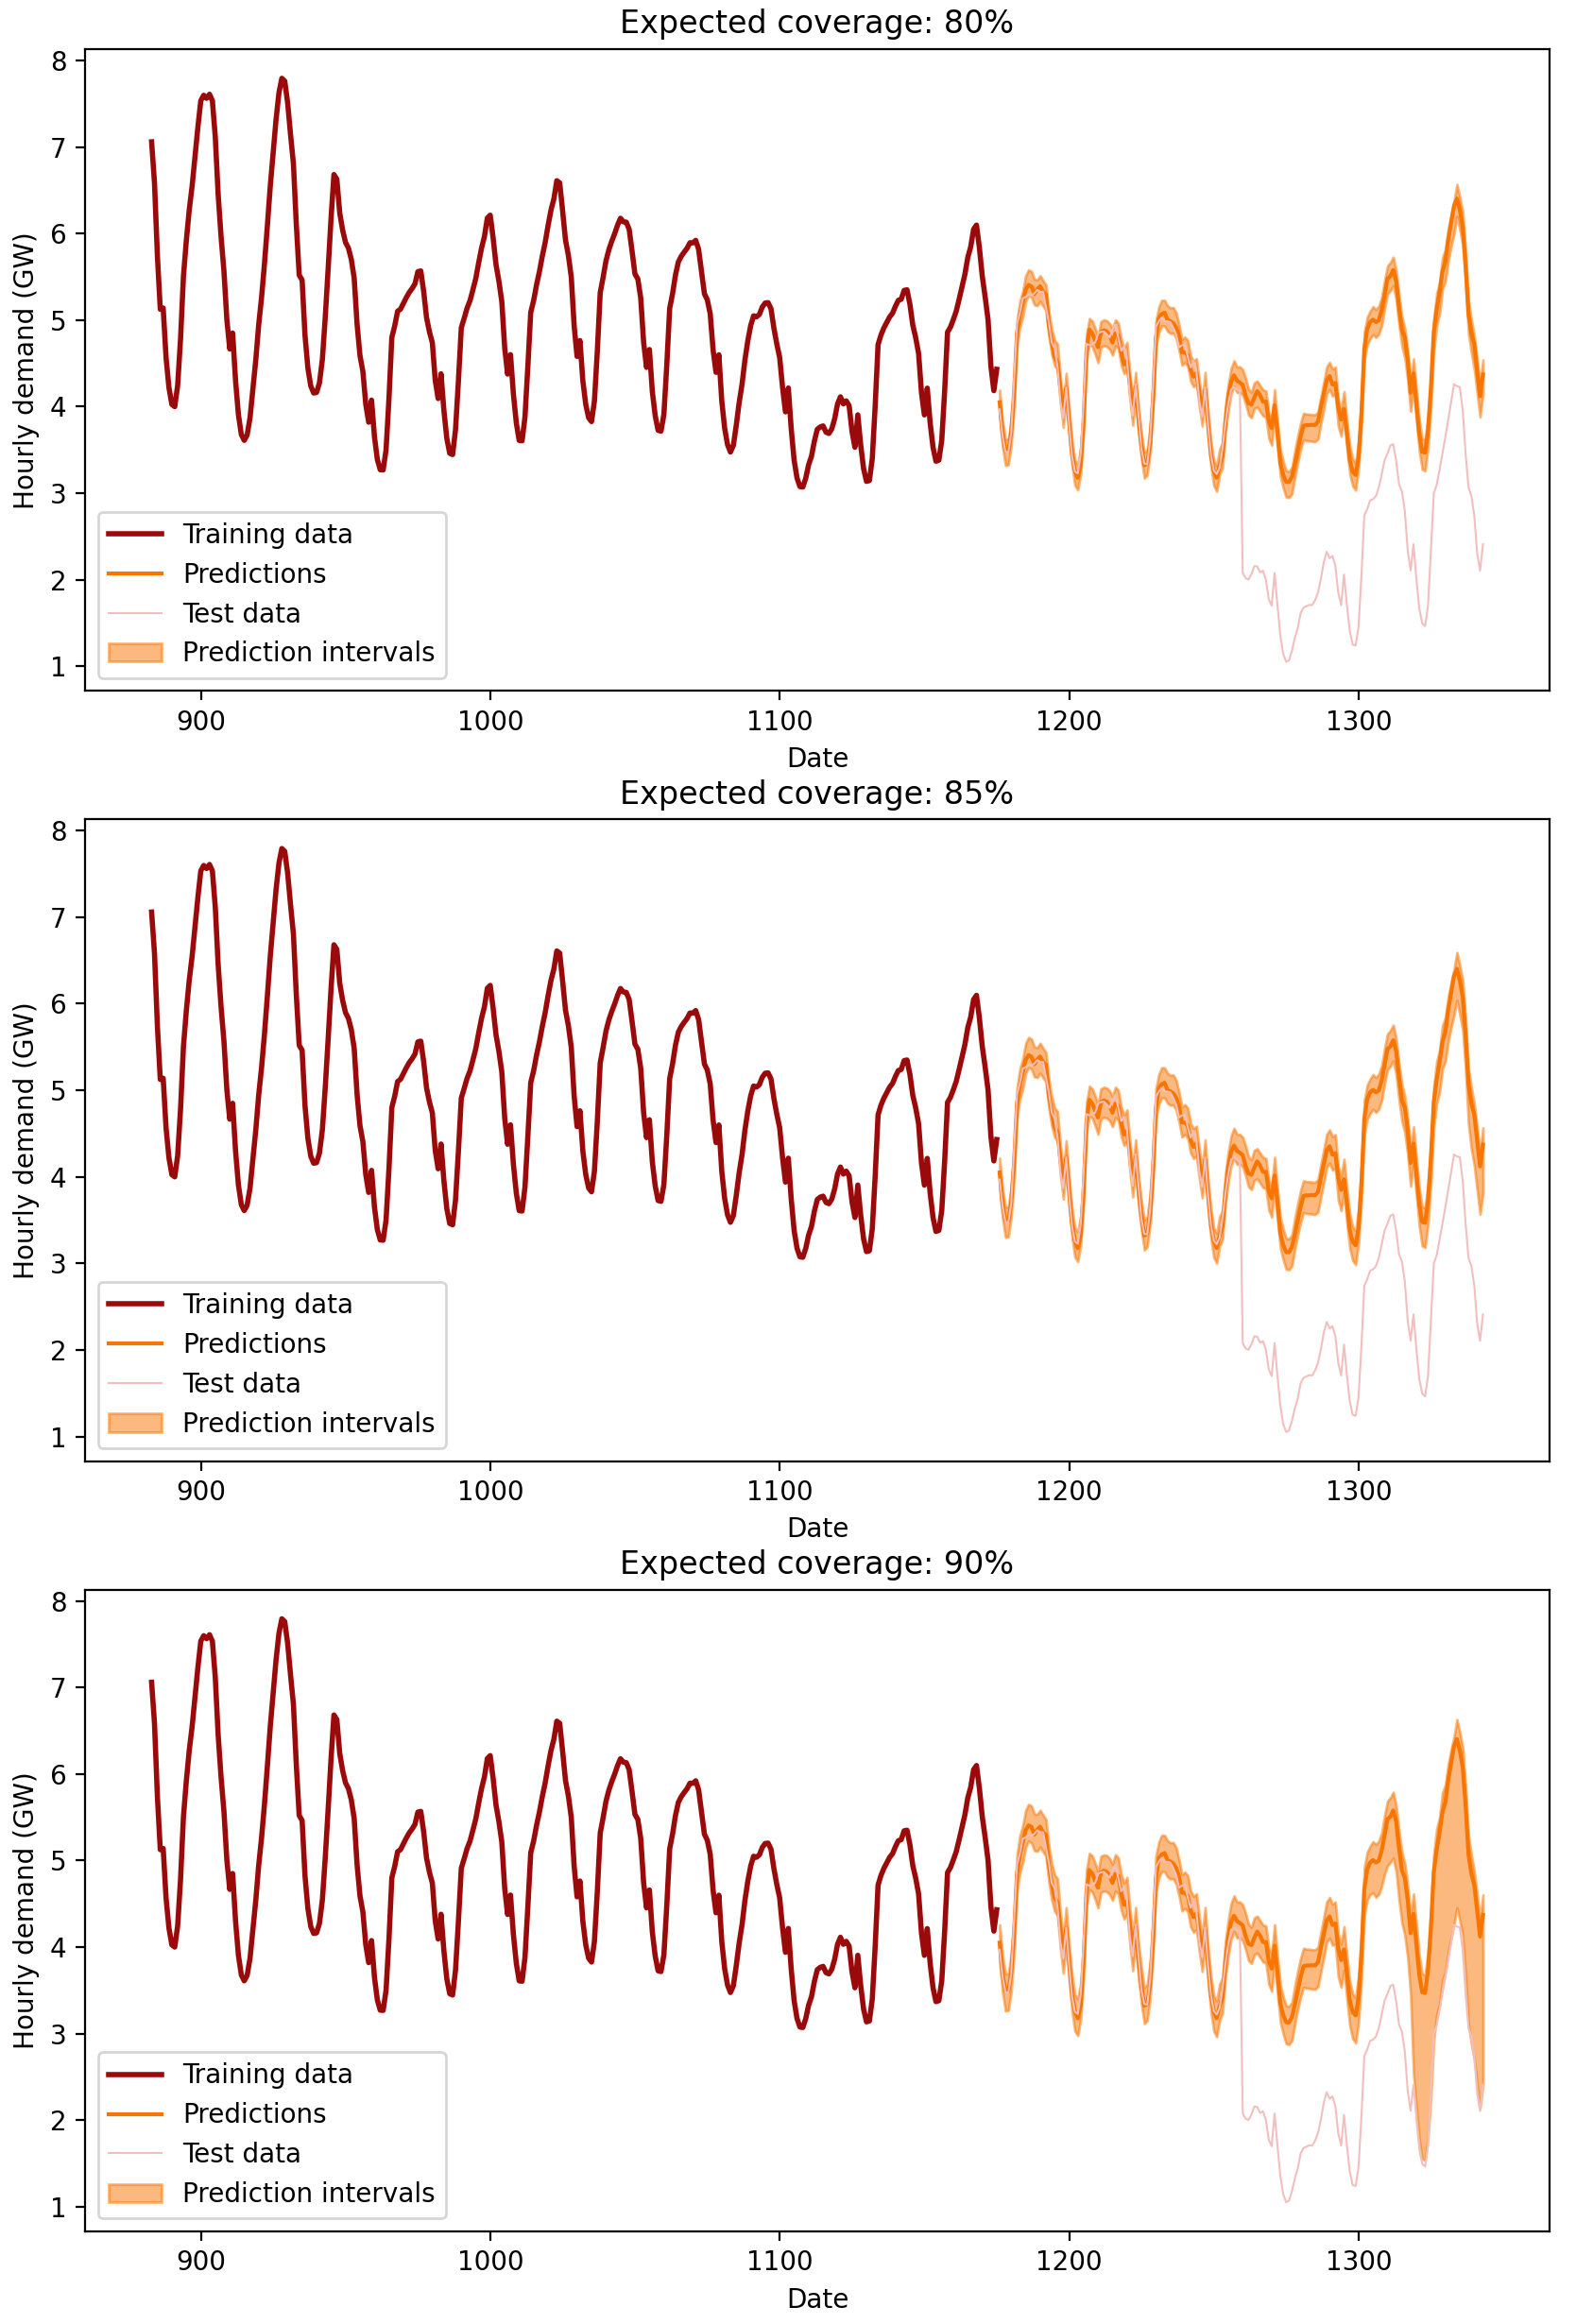
\includegraphics[width=0.6\textwidth, height=0.6\textwidth]{Figures/timeseries/with-change-point/prediction-intervals-in-function-of-miscoverage.png}
%     \caption{EnbPI recovering intervals' width for $\a=0.20, 0.15, 0.10$.}
%     % \label{fig:timeseries-intervals-alpha-cpoint}
% \end{figure}

% \end{frame}

%%% Conclusions %%% (2pp)

\section{Conclusions}

% Regression & time series %

\begin{frame}{Regression \& time series}
\begin{itemize}%[<+->][<+->]
    \item[] The best strategies for exchangeable data are, \textbf{decreasingly ordered} by:
    \begin{itemize}%[<+->][<+->]
        \item \textit{Statistical efficiency}: CQR, SCP, CV$+$, J$+$aB.
        \begin{itemize}%[<+->]
            \item This is fulfilled independently of $\a$.
        \end{itemize}
        \item \textit{Computational efficiency}: SCP, CQR, CV$+$, J$+$aB.
        \item \textit{Predictive power} are: CV$+$ \& J$+$aB, SCP, CQR.
        \item "\textit{Informativeness}": J$+$aB, SCP, CQR, CV$+$.
        \item \textit{Adaptability}: CQR, CV$+$, J$+$aB (slight to none). Contrarily, SCP intervals are not adaptive at all. 
    \end{itemize}
    \item[] Regarding the time series case, \textbf{EnbPI} is a \textbf{suitable option} to provide valid intervals.
    \begin{itemize}%[<+->][<+->]
        \item EnbPI's adjustment using test residuals is necessary.
        \item This option also allows all the issued \textbf{intervals} to be \textbf{adaptive}.
    \end{itemize}
        
\end{itemize}
\end{frame}

% % Further research %

% \begin{frame}{Further research}
% Some of the next possible research lines are: 
%     \begin{itemize}%[<+->][<+->]
%         \item Leverage cross-validation folds in the CQR strategy, instead of a simple train-test split of the dataset.
%         \item Implement other contemporary CP methodologies for time series problems, such as \texttt{ACI} (\cite{gibbs2021}) \& \texttt{HopCPT} (\cite{auer2023}).
%         \item Extend all these methods to the multi-dimensional output variables' case (regression \& time series problems).
%         \item Apply the former methodologies to classification problems.
%     \end{itemize}
% \end{frame}

%%%% CLOSING SLIDE %%%%
\section*{}
\begin{frame}[noframenumbering]
\vspace{1cm}
\begin{center}
    {\Huge Thank you for your attention!} \\ 
    \vspace{1cm}
    {\normalsize Questions?}
\end{center}

\end{frame}

% \begin{frame}{Pros \& cons}
%     \begin{table}[ht]
%     \centering
%     \begin{tabularx}{\linewidth}{@{}X>{\hsize=.85\hsize}X>{\hsize=.5\hsize}X@{}}
%     \toprule
%     \textbf{Pros} & \textbf{Cons} \\ \midrule
%     Significant gain in metrics & Not useful in many tasks (annotated data needed) \\
%     Does not require different data & Higher layers can now just focus on 1 part \\
%     Loss function not changed & Lower layers interpretability not assessed \\
%     Applicable to several architectures & Filter-category mapping not injective \\
%      & Assigned category can change mid-training \\
%      & Training process more expensive \& complex \\
%     \bottomrule
%     \end{tabularx}
%     % \caption{Pros and cons}
%     % \label{table:pros_cons}
%     \end{table}
% \end{frame}

% % BIBLIOGRAPHY

% %\printbibliography%[heading=bibintoc]

\end{document}